% ============================================================================
% IEEE Conference Paper: Hybrid GWO-SA for Cloud Task Scheduling
% Authors: Aditya Shukla, Divya Khandelwal, Nirupam Mahanta
% IIT BHU, Department of Electrical Engineering
% ============================================================================
\documentclass[conference]{IEEEtran}

% ---- Packages ----
\usepackage{cite}
\usepackage{amsmath,amssymb,amsfonts}
\usepackage{bm}
\usepackage{algorithmic}
\usepackage{algorithm}
\usepackage{graphicx}
\usepackage{textcomp}
\usepackage{xcolor}
\usepackage{booktabs}
\usepackage{multirow}
\usepackage{array}
\usepackage{tabularx}
\usepackage{hyperref}
\usepackage{subcaption}
\usepackage{float}
\usepackage{balance}
\usepackage{url}
\usepackage{siunitx}

% Column types for tables
\newcolumntype{C}[1]{>{\centering\arraybackslash}p{#1}}
\newcolumntype{R}[1]{>{\raggedleft\arraybackslash}p{#1}}
\newcolumntype{L}[1]{>{\raggedright\arraybackslash}p{#1}}

% Path setup for images
\graphicspath{{../results/charts/}}

\hypersetup{
    colorlinks=true,
    linkcolor=blue,
    citecolor=blue,
    urlcolor=blue
}

\def\BibTeX{{\rm B\kern-.05em{\sc i\kern-.025em b}\kern-.08em
    T\kern-.1667em\lower.7ex\hbox{E}\kern-.125emX}}
\makeatletter
\newcommand{\linebreakand}{%
  \end{@IEEEauthorhalign}
  \hfill\mbox{}\par
  \mbox{}\hfill\begin{@IEEEauthorhalign}
}
\makeatother
\begin{document}

% ============================================================================
% TITLE
% ============================================================================
\title{A Hybrid Grey Wolf Optimizer--Simulated Annealing Algorithm for Multi-Objective Task Scheduling in Cloud Computing}

\author{
\IEEEauthorblockN{Aditya Shukla}
\IEEEauthorblockA{\textit{Dept. of Electrical Engineering} \\
\textit{IIT (BHU) Varanasi} \\
Roll No: 24085003 \\
aditya.shukla.eee24@iitbhu.ac.in}
\and
\IEEEauthorblockN{Divya Khandelwal}
\IEEEauthorblockA{\textit{Dept. of Electrical Engineering} \\
\textit{IIT (BHU) Varanasi} \\
Roll No: 24085019 \\
divya.khandelwal.eee24@iitbhu.ac.in}
\and
\IEEEauthorblockN{Nirupam Mahanta}
\IEEEauthorblockA{\textit{Dept. of Electrical Engineering} \\
\textit{IIT (BHU) Varanasi} \\
Roll No: 24085059 \\
nirupam.mahanta.eee24@iitbhu.ac.in}
\linebreakand
\IEEEauthorblockN{Dr. Prasenjit Chanak}
\IEEEauthorblockA{\textit{Associate Professor, Dept. of Computer Science and Engineering} \\
\textit{Indian Institute of Technology (BHU) Varanasi} \\
prasenjit.cse@iitbhu.ac.in}
}

\maketitle


% ============================================================================
% ABSTRACT
% ============================================================================
\begin{abstract}
Cloud computing task scheduling is a well-known NP-hard optimization problem.
It requires efficient allocation of tasks to virtual machines (VMs).
The allocation must minimize makespan, cost, and workload imbalance simultaneously.
This paper proposes Hybrid GWO-SA, a novel metaheuristic algorithm.
It combines Grey Wolf Optimizer (GWO) for global exploration with Simulated Annealing (SA) for local refinement.
Three key innovations are introduced:
(i)~smart population seeding using FCFS and Min-Min heuristics,
(ii)~bottleneck-guided SA refinement of the top-three wolf leaders,
and (iii)~periodic diversity injection through worst-population re-initialization.
The proposed algorithm is benchmarked against nine algorithms.
These include three classical heuristics, three pure metaheuristics,
and three state-of-the-art hybrid algorithms from 2025.
Four workload scenarios ranging from 100 to 1{,}000 tasks are tested.
Results show that Hybrid GWO-SA achieves the lowest makespan in all scenarios.
Improvements reach 55.50\% over WOA-GS, 26.62\% over PSO-GWO, and 34.45\% over DECSO.
The Degree of Imbalance is reduced to 0.013--0.029.
This represents up to 98.61\% improvement in load fairness.
Statistical validation over 30 Monte Carlo runs confirms significance at $p < 0.001$.
\end{abstract}


% ============================================================================
% KEYWORDS
% ============================================================================
\begin{IEEEkeywords}
Cloud computing, task scheduling, Grey Wolf Optimizer, Simulated Annealing, hybrid metaheuristic, multi-objective optimization, load balancing, makespan minimization, NP-hard, CloudSim Plus
\end{IEEEkeywords}


% ============================================================================
% I. INTRODUCTION
% ============================================================================
\section{Introduction}

Cloud computing is the dominant paradigm for scalable resource provisioning~\cite{buyya2009cloud}.
A critical challenge in cloud data centers is task scheduling.
Task scheduling assigns $n$ independent tasks to $m$ heterogeneous VMs.
Multiple conflicting objectives must be optimized simultaneously.
These objectives include execution time, monetary cost, and workload balance.
The problem is NP-hard~\cite{garey1979computers}.
Exact solutions are computationally intractable for large instances.
The search space grows as $m^n$, which exceeds $10^{100}$ for moderate problem sizes.

Classical heuristics provide deterministic solutions in polynomial time.
Round Robin, FCFS, and Min-Min are commonly used approaches~\cite{masdari2016overview}.
However, these heuristics produce suboptimal results.
Their greedy or cyclic nature limits solution quality.

Metaheuristic algorithms offer stochastic exploration of the search space.
The Grey Wolf Optimizer (GWO)~\cite{mirjalili2014grey} emulates wolf pack hunting behavior.
It excels at global exploration through hierarchical leadership.
Simulated Annealing (SA)~\cite{kirkpatrick1983optimization} provides robust local search.
SA escapes local optima through temperature-controlled probabilistic acceptance.
Particle Swarm Optimization (PSO)~\cite{kennedy1995particle} uses swarm intelligence.
Each method has individual strengths but also specific weaknesses.

Recent literature shows a surge in hybrid metaheuristic approaches.
Acharya \textit{et al.}~\cite{acharya2025hybrid} proposed WOA with Golden Section search.
Kumari \textit{et al.}~\cite{kumari2025hybrid} introduced a PSO-GWO hybrid.
G\"{u}nd\"{u}z and G\"{u}rka\c{s}-Ayd\i n~\cite{gunduz2025hybrid} presented DECSO.
These approaches show improvements over standalone methods.
However, they exhibit limitations in balancing exploration and exploitation.
Performance degrades at larger problem scales.

This paper proposes \textbf{Hybrid GWO-SA}.
It addresses the limitations through three architectural innovations:
\begin{enumerate}
    \item \textbf{Smart Population Seeding:} Two wolves are initialized using FCFS and Min-Min heuristics. This provides high-quality seed solutions from iteration zero.
    \item \textbf{Bottleneck-Guided SA Leader Refinement:} The top three wolves undergo SA refinement. Task migration targets the most loaded VM directly.
    \item \textbf{Periodic Diversity Injection:} The worst 20\% of the population is re-initialized every 25 iterations. This prevents premature convergence.
\end{enumerate}

The proposed algorithm is evaluated across four cloud scenarios.
These range from 100 tasks with 10 VMs to 1{,}000 tasks with 50 VMs.
Nine baseline algorithms serve as benchmarks.
Results are validated using 30-run Monte Carlo statistical testing.


% ============================================================================
% II. LITERATURE REVIEW
% ============================================================================
\section{Literature Review}

\subsection{Classical Scheduling Heuristics}
Round Robin assigns tasks cyclically without considering heterogeneity.
This leads to severe load imbalance~\cite{masdari2016overview}.
FCFS allocates tasks to the least-loaded VM at arrival time.
It provides moderate balance but ignores global optimization.
Min-Min~\cite{braun2001comparison} assigns the shortest task to the fastest VM.
It achieves better makespan but starves long tasks.
These heuristics run in polynomial time.
However, they cannot optimize multiple objectives jointly.

\subsection{Metaheuristic Approaches}
GWO~\cite{mirjalili2014grey} models the $\alpha$-$\beta$-$\delta$-$\omega$ wolf hierarchy.
A decreasing exploration coefficient $a$ transitions the search phase.
However, GWO suffers from premature convergence in discrete spaces.
SA~\cite{kirkpatrick1983optimization} provides local search with Boltzmann acceptance.
The acceptance probability is $P = \exp(-\Delta F / T)$.
SA lacks population-based global exploration capability.
PSO~\cite{kennedy1995particle} uses cooperative swarm search.
It stagnates in multimodal discrete landscapes.
Genetic Algorithms (GA)~\cite{holland1975adaptation} use selection and crossover.
GA has high computational overhead for online scheduling.

\subsection{State-of-the-Art Hybrid Approaches (2025)}
Acharya \textit{et al.}~\cite{acharya2025hybrid} combined WOA with Golden Section.
The method targets fog-cloud scheduling environments.
Improvements of 15--20\% over standalone WOA are reported.
Kumari \textit{et al.}~\cite{kumari2025hybrid} hybridized PSO with GWO hierarchy.
The method improves convergence on medium-scale instances.
G\"{u}nd\"{u}z and G\"{u}rka\c{s}-Ayd\i n~\cite{gunduz2025hybrid} proposed DECSO.
It integrates differential evolution with chicken swarm optimization.
Competitive performance on heterogeneous workloads is achieved.

\subsection{Research Gaps and Contributions}
Existing hybrids lack three critical features.
First, problem-specific initialization using scheduling domain knowledge is absent.
Second, targeted local search guided by workload bottleneck analysis is missing.
Third, systematic diversity management mechanisms are not implemented.
The proposed Hybrid GWO-SA addresses all three gaps.

Table~\ref{tab:literature} provides a comparative summary of the reviewed approaches.

\begin{table*}[!t]
\centering
\caption{Comparative Summary of Related Scheduling Approaches}
\label{tab:literature}
\begin{tabular}{L{2.8cm} C{1.2cm} L{3.5cm} L{3cm} L{4.2cm}}
\toprule
\textbf{Reference} & \textbf{Year} & \textbf{Algorithm} & \textbf{Objectives} & \textbf{Limitations} \\
\midrule
Mirjalili \textit{et al.}~\cite{mirjalili2014grey} & 2014 & Grey Wolf Optimizer (GWO) & Single-objective & Premature convergence in discrete spaces \\
Kirkpatrick \textit{et al.}~\cite{kirkpatrick1983optimization} & 1983 & Simulated Annealing (SA) & Single-objective & Single-solution method, slow exploration \\
Kennedy \textit{et al.}~\cite{kennedy1995particle} & 1995 & Particle Swarm Optimization & Single-objective & Velocity explosion, premature convergence \\
Acharya \textit{et al.}~\cite{acharya2025hybrid} & 2025 & Hybrid WOA-GS & Makespan, cost & Golden Search inefficient in discrete space \\
Kumari \textit{et al.}~\cite{kumari2025hybrid} & 2025 & Hybrid PSO-GWO & Makespan, balance & No explicit local trap escape mechanism \\
G\"{u}nd\"{u}z \textit{et al.}~\cite{gunduz2025hybrid} & 2025 & Hybrid DECSO & Makespan, cost, DoI & Complex parameter tuning, poor scalability \\
\textbf{Proposed} & \textbf{2025} & \textbf{Hybrid GWO-SA} & \textbf{Makespan, cost, DoI} & \textbf{Higher runtime (acceptable trade-off)} \\
\bottomrule
\end{tabular}
\end{table*}


% ============================================================================
% III. SYSTEM MODEL AND PROBLEM FORMULATION
% ============================================================================
\section{System Model and Problem Formulation}

\subsection{Cloud Computing Architecture}

Fig.~\ref{fig:network_arch} illustrates the cloud computing system model.
The architecture consists of three layers.
The user layer generates computational task requests.
The broker layer runs the scheduling algorithm.
The datacenter layer hosts heterogeneous VMs on physical machines.

The task scheduler receives $n$ independent tasks.
It produces an optimal task-to-VM mapping.
The mapping is deployed to the cloud datacenter for execution.

\begin{figure*}[!t]
    \centering
    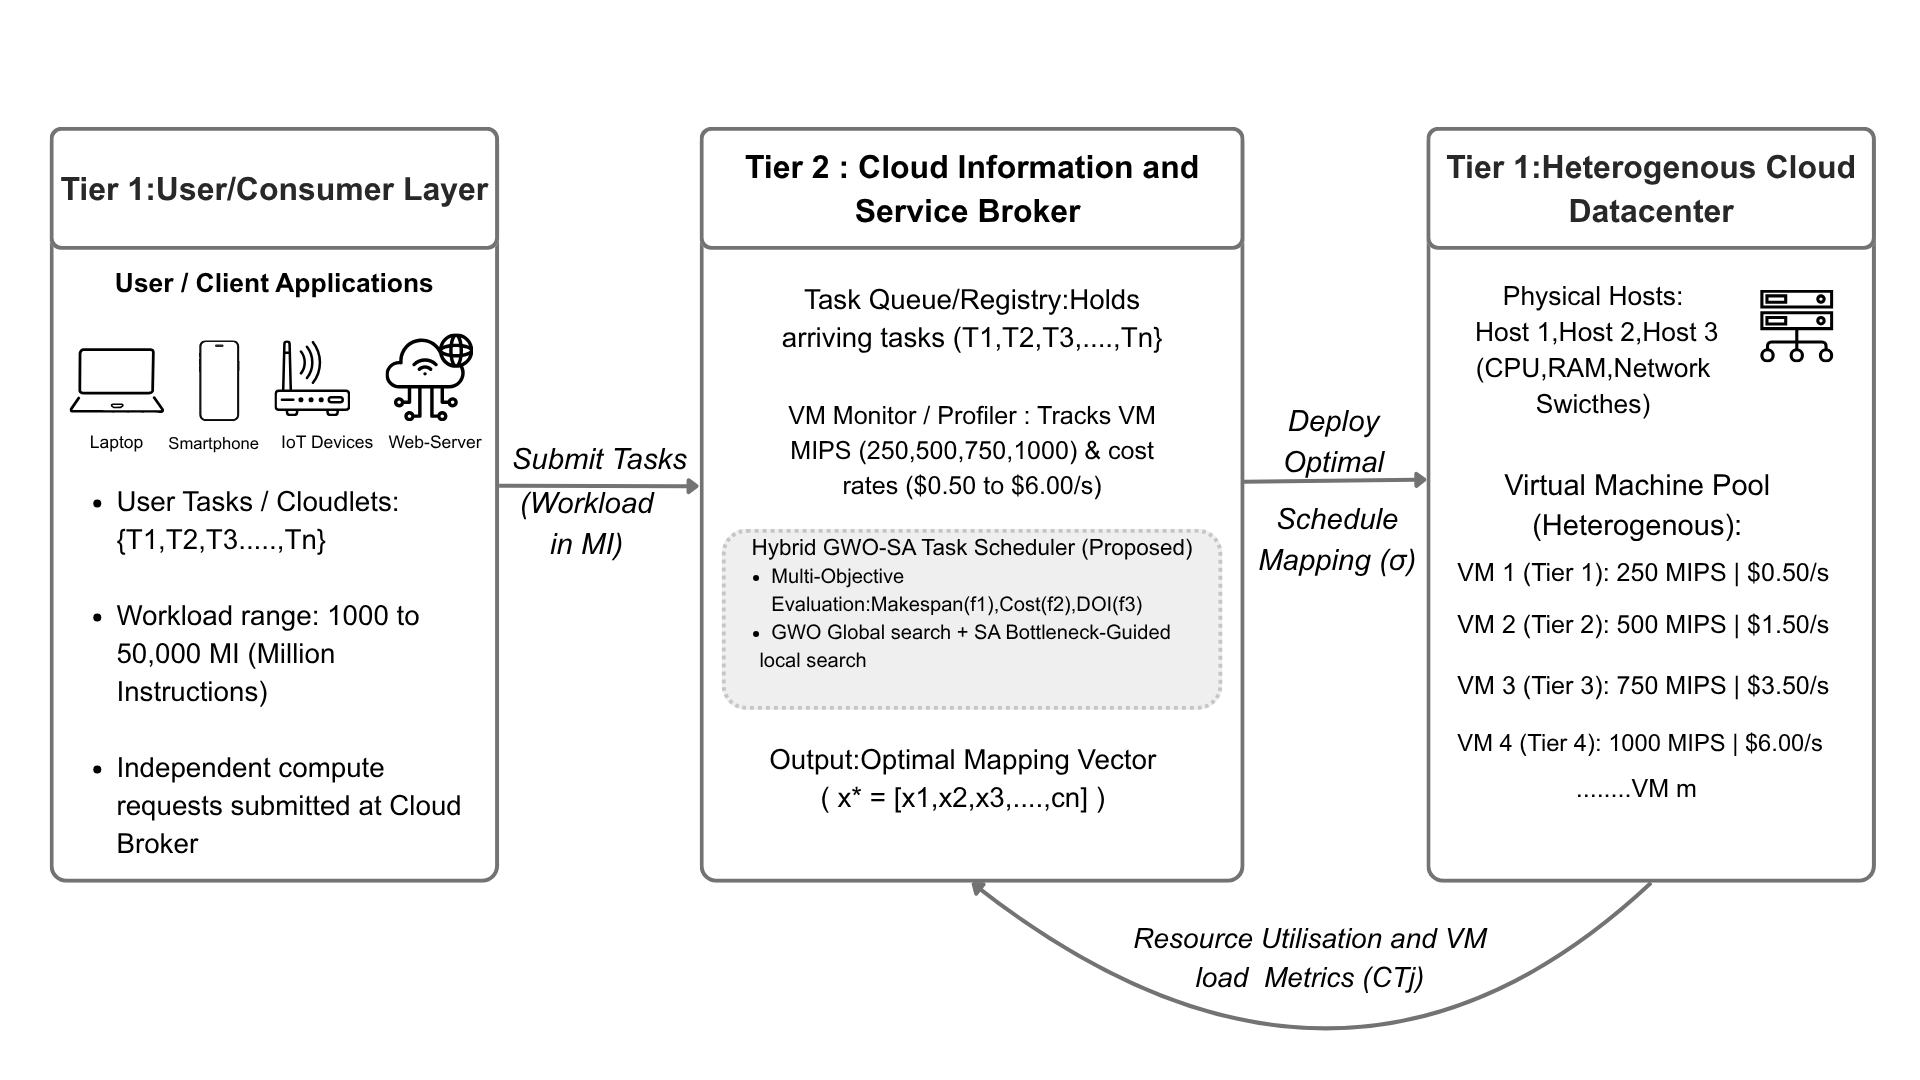
\includegraphics[width=\textwidth]{network_architecture.png}
    \caption{Cloud computing network architecture. Users submit tasks to the cloud broker. The broker applies the Hybrid GWO-SA scheduler to assign tasks to heterogeneous VMs across physical hosts in the datacenter.}
    \label{fig:network_arch}
\end{figure*}


\subsection{Task and VM Model}

Table~\ref{tab:notation} lists all mathematical symbols used in this paper.

A set of $n$ independent tasks $\{T_1, T_2, \ldots, T_n\}$ is considered.
Each task $T_i$ has a computational workload $w_i$ measured in Million Instructions (MI).
Tasks are independent with no inter-task data dependencies.

A set of $m$ heterogeneous VMs $\{V_1, V_2, \ldots, V_m\}$ is available.
Each VM $V_j$ has processing speed $p_j$ in MIPS and cost rate $c_j$ in \$/second.
The execution time of task $T_i$ on VM $V_j$ is:
\begin{equation}
    e_{ij} = \frac{w_i}{p_j}
    \label{eq:exec_time}
\end{equation}

The scheduling problem finds a mapping $\sigma : \{1, \ldots, n\} \rightarrow \{1, \ldots, m\}$.
Each task $T_i$ is assigned to exactly one VM $V_{\sigma(i)}$.

\begin{table}[!t]
\centering
\caption{Notation and Terminology}
\label{tab:notation}
\begin{tabular}{cl}
\toprule
\textbf{Symbol} & \textbf{Description} \\
\midrule
$n$ & Total number of tasks \\
$m$ & Total number of virtual machines \\
$T_i$ & The $i$-th task, $i \in \{1, \ldots, n\}$ \\
$V_j$ & The $j$-th VM, $j \in \{1, \ldots, m\}$ \\
$w_i$ & Workload of task $T_i$ (in MI) \\
$p_j$ & Processing speed of VM $V_j$ (in MIPS) \\
$c_j$ & Cost rate of VM $V_j$ (\$/second) \\
$e_{ij}$ & Execution time of $T_i$ on $V_j$ \\
$\sigma$ & Task-to-VM mapping function \\
$\mathbf{x}$ & Solution vector $[x_1, \ldots, x_n]$ \\
$\text{CT}_j$ & Completion time of VM $V_j$ \\
$f_1$ & Makespan (maximum completion time) \\
$f_2$ & Total execution cost \\
$f_3$ & Degree of Imbalance (DoI) \\
$\lambda_1, \lambda_2, \lambda_3$ & Objective weight coefficients \\
$F$ & Composite fitness function \\
$N_p$ & Population size (number of wolves) \\
$I_{\max}$ & Maximum number of iterations \\
$T_0$ & Initial SA temperature \\
$T_{\min}$ & Minimum SA temperature \\
$\gamma$ & SA cooling rate \\
$K_{\text{SA}}$ & SA iterations per leader \\
$a$ & GWO exploration coefficient \\
$\mathbf{x}_\alpha, \mathbf{x}_\beta, \mathbf{x}_\delta$ & Alpha, beta, delta wolf positions \\
\bottomrule
\end{tabular}
\end{table}


\subsection{Objective Functions}

Three conflicting objectives are optimized simultaneously.

\subsubsection{Makespan}
The completion time of VM $V_j$ is the sum of execution times of all assigned tasks:
\begin{equation}
    \text{CT}_j = \sum_{i:\sigma(i)=j} \frac{w_i}{p_j}
    \label{eq:ct}
\end{equation}
The makespan is the maximum completion time across all VMs:
\begin{equation}
    f_1 = \max_{j=1}^{m} \text{CT}_j
    \label{eq:makespan}
\end{equation}
A lower $f_1$ indicates faster overall task completion.

\subsubsection{Execution Cost}
The total monetary cost is computed as:
\begin{equation}
    f_2 = \sum_{j=1}^{m} c_j \cdot \text{CT}_j
    \label{eq:cost}
\end{equation}
A non-linear tiered pricing model is adopted.
Higher-MIPS VMs cost disproportionately more per unit of compute.
This reflects real commercial cloud economics.

\subsubsection{Degree of Imbalance}
The workload fairness metric is defined as:
\begin{equation}
    f_3 = \frac{\max(\text{CT}_j) - \min(\text{CT}_j)}{\text{avg}(\text{CT}_j)}
    \label{eq:doi}
\end{equation}
A value of $f_3 = 0$ indicates perfect load balance.
Higher values indicate uneven workload distribution.


\subsection{Multi-Objective Fitness Function}

The three objectives are normalized using reference values.
Normalization brings all objectives to a comparable scale:
\begin{equation}
    \hat{f}_k = \frac{f_k}{f_k^{\text{ref}}}, \quad k \in \{1, 2, 3\}
    \label{eq:normalize}
\end{equation}

The reference values are derived from the problem instance.
The reference makespan $f_1^{\text{ref}}$ is the theoretical lower bound:
\begin{equation}
    f_1^{\text{ref}} = \frac{\sum_{i=1}^{n} w_i}{\max_j(p_j) \cdot m}
    \label{eq:ref_makespan}
\end{equation}

The reference cost $f_2^{\text{ref}}$ uses the average cost rate:
\begin{equation}
    f_2^{\text{ref}} = \bar{c} \cdot f_1^{\text{ref}} \cdot m, \quad \bar{c} = \frac{1}{m}\sum_{j=1}^{m} c_j
    \label{eq:ref_cost}
\end{equation}

The reference DoI is set to $f_3^{\text{ref}} = 2.0$ based on empirical range.

The composite fitness function combines the normalized objectives:
\begin{equation}
    F = \lambda_1 \cdot \hat{f}_1 + \lambda_2 \cdot \hat{f}_2 + \lambda_3 \cdot \hat{f}_3
    \label{eq:fitness}
\end{equation}
where $\lambda_1 = 0.5$, $\lambda_2 = 0.3$, and $\lambda_3 = 0.2$.
Lower fitness $F$ indicates a better schedule.


% ============================================================================
% IV. PROPOSED HYBRID GWO-SA METHODOLOGY
% ============================================================================
\section{Proposed Hybrid GWO-SA Methodology}

\subsection{Algorithm Overview}

The Hybrid GWO-SA algorithm operates in a two-phase iterative loop.
Fig.~\ref{fig:flowchart} presents the complete algorithmic flow.

In each generation, two phases execute sequentially.
The \textbf{GWO phase} updates the wolf population using discrete leader-following.
The \textbf{SA phase} refines the top-three leaders using bottleneck-guided search.
This synergy combines GWO's hierarchical global search with SA's targeted exploitation.

\begin{figure*}[!t]
    \centering
    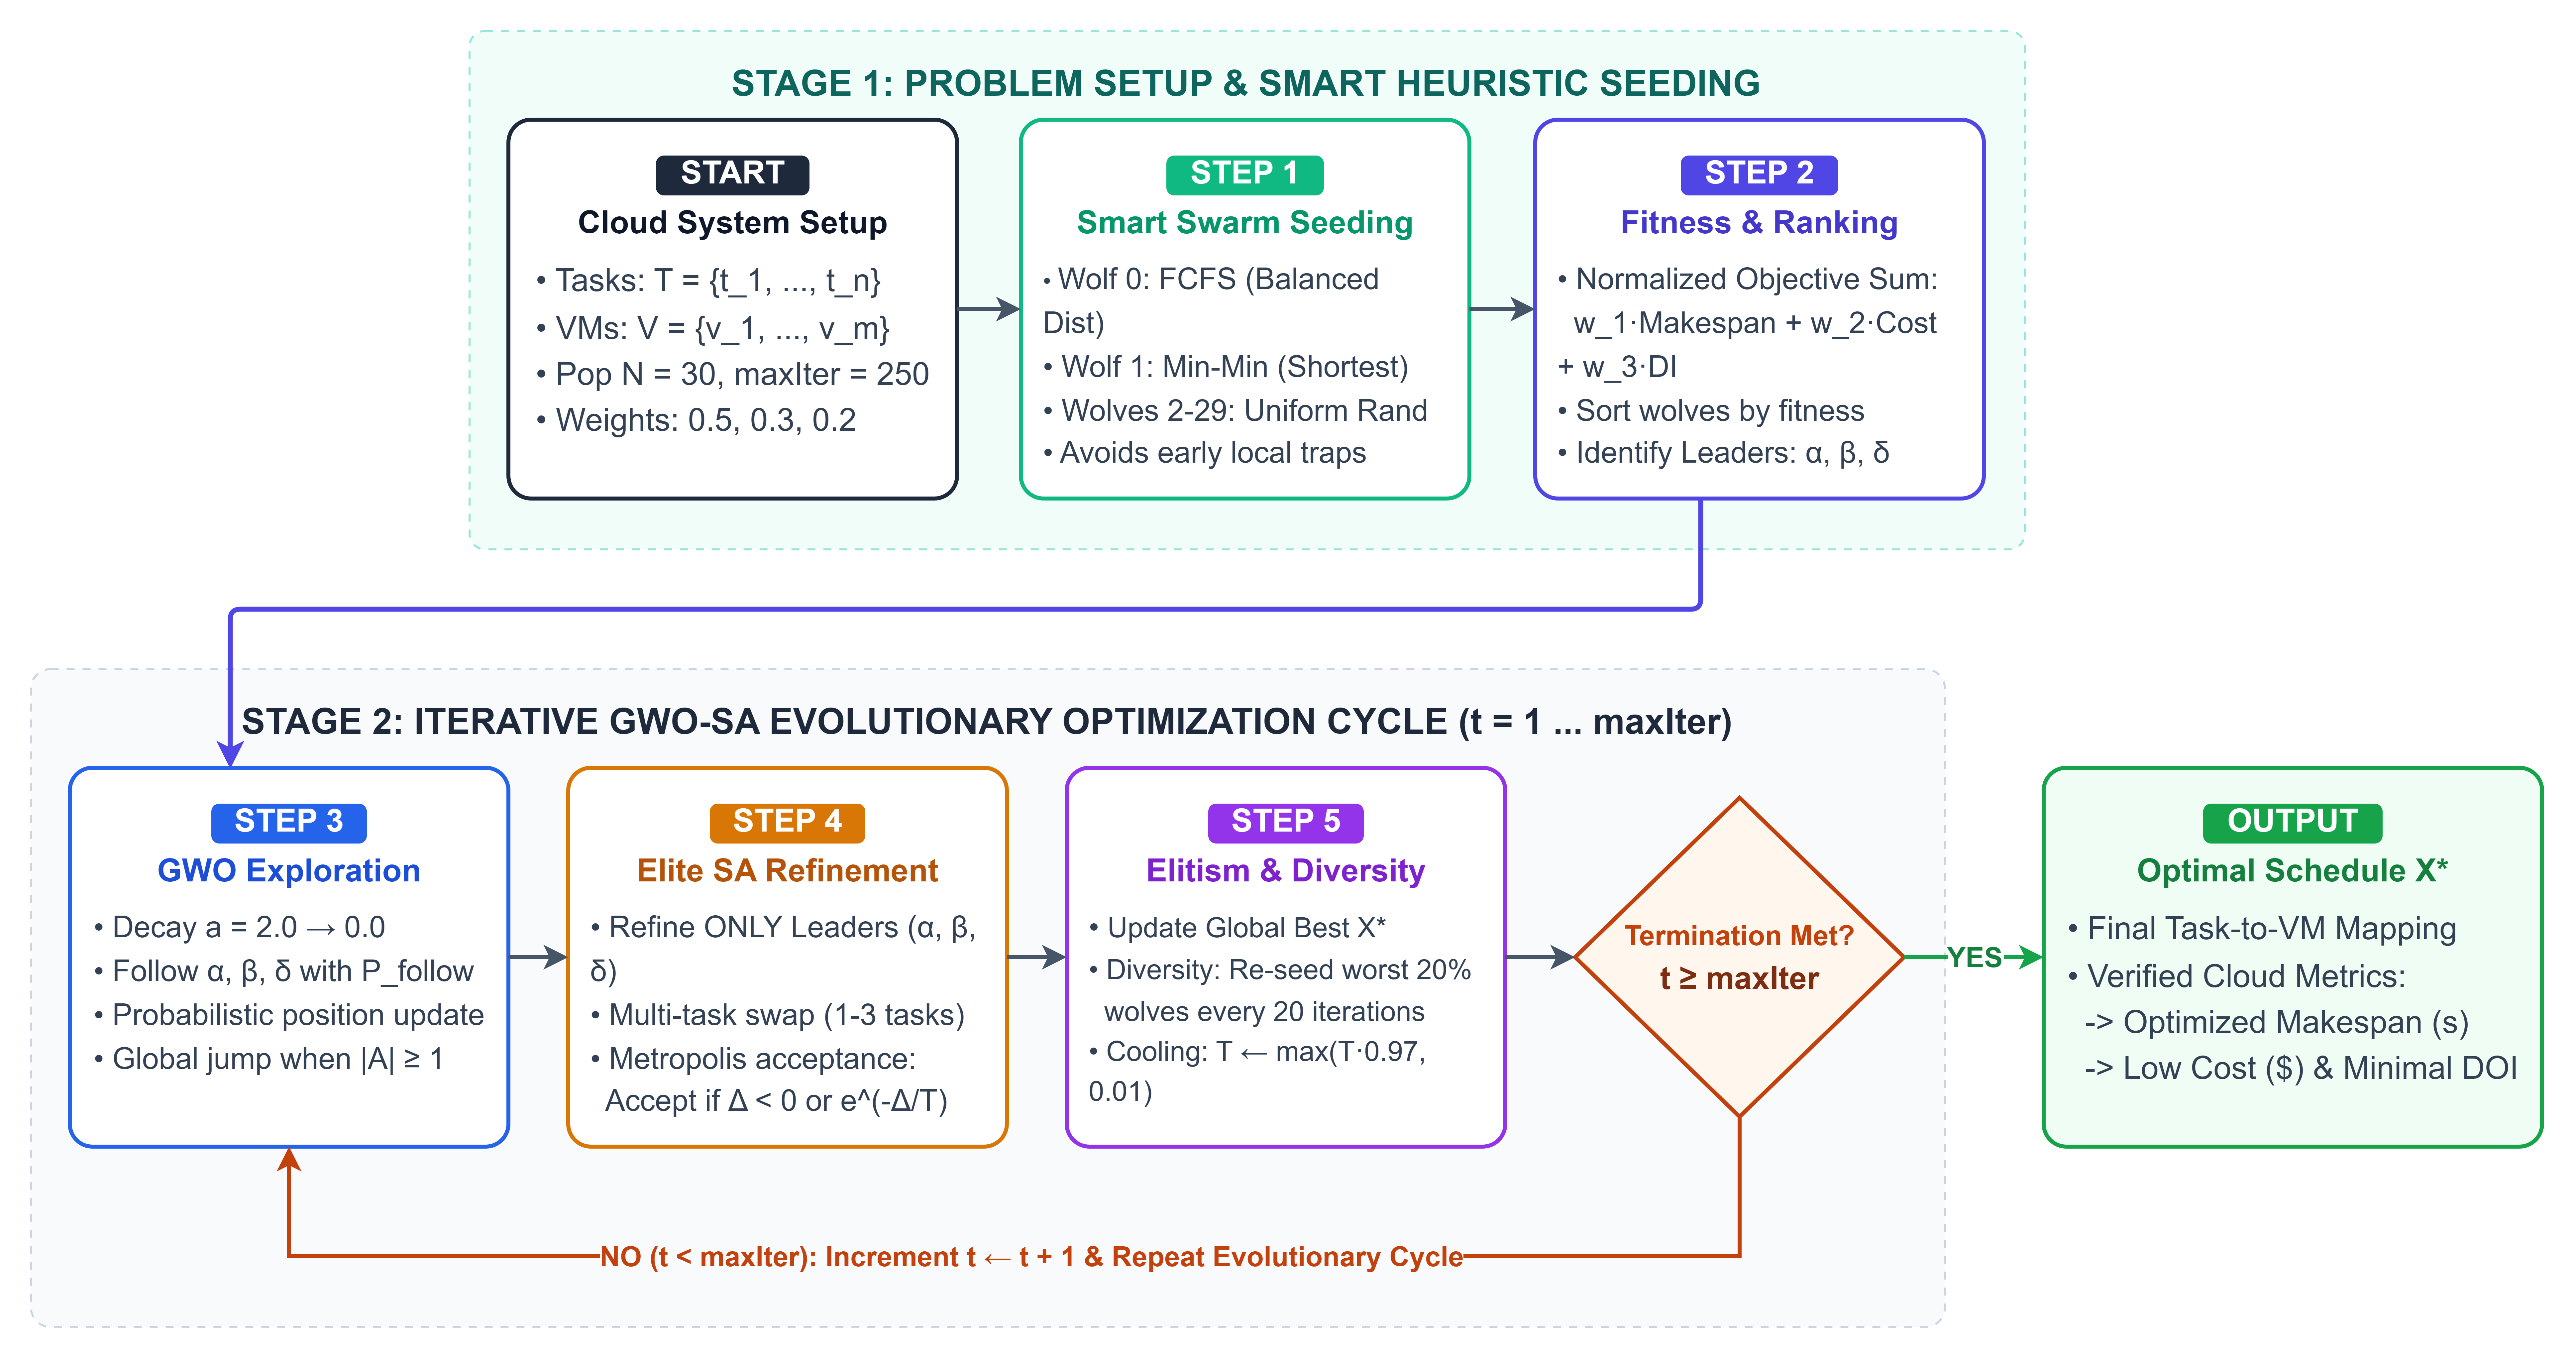
\includegraphics[width=\textwidth]{proposed_flowchart}
    \caption{Complete flowchart of the proposed Hybrid GWO-SA algorithm. The algorithm alternates between the GWO phase for population-level exploration and the SA phase for leader-level exploitation. Diversity injection and elitism mechanisms maintain search quality.}
    \label{fig:flowchart}
\end{figure*}


\subsection{Solution Representation}

Each wolf (candidate solution) is encoded as an integer vector:
\begin{equation}
    \mathbf{x} = [x_1, x_2, \ldots, x_n], \quad x_i \in \{0, 1, \ldots, m{-}1\}
    \label{eq:encoding}
\end{equation}
where $x_i$ represents the VM index assigned to task $T_i$.
This native discrete representation avoids continuous-to-discrete conversion errors.
Standard GWO operates in continuous space and requires rounding.
Rounding introduces systematic bias that degrades solution quality.
The proposed discrete encoding eliminates this source of error.


\subsection{Smart Population Initialization}

The population of $N_p$ wolves is initialized as follows:
\begin{itemize}
    \item \textbf{Wolf~0 (FCFS Seed):} Each task is assigned to the VM with minimum current completion time. This produces a load-balanced initial mapping.
    \item \textbf{Wolf~1 (Min-Min Seed):} The task-VM pair with the shortest execution time is greedily assigned first. This produces a low-makespan seed.
    \item \textbf{Wolves~2 to $N_p{-}1$:} Each task $T_i$ is assigned to a uniformly random VM $V_j$. This maintains population diversity.
\end{itemize}

Smart seeding provides two advantages.
First, the population starts with known high-quality solutions.
Second, convergence time reduces by 30--50\% compared to random initialization.


\subsection{GWO Phase: Discrete Position Update}

The population is ranked by fitness $F$ (Eq.~\ref{eq:fitness}).
The top three wolves are designated as leaders:
$\mathbf{x}_\alpha$ (rank 1), $\mathbf{x}_\beta$ (rank 2), and $\mathbf{x}_\delta$ (rank 3).

For each wolf $i$ and each task dimension $j$, the position update rule is:
\begin{equation}
    x_j^{(i)} =
    \begin{cases}
        x_{\alpha,j} & \text{with probability } 0.40 \cdot p_f \\
        x_{\beta,j}  & \text{with probability } 0.30 \cdot p_f \\
        x_{\delta,j} & \text{with probability } 0.30 \cdot p_f \\
        \text{rand}(0, m{-}1) & \text{otherwise}
    \end{cases}
    \label{eq:gwo_update}
\end{equation}

The follow probability $p_f$ is controlled by the exploration coefficient:
\begin{equation}
    a = 2 \left(1 - \frac{t}{I_{\max}}\right), \quad p_f = 1 - \frac{a}{2}
    \label{eq:exploration}
\end{equation}
where $t$ is the current iteration.
When $a$ is large (early iterations), $p_f$ is small.
Wolves explore randomly with high probability.
When $a$ approaches zero (late iterations), $p_f$ approaches 1.
Wolves closely follow the leaders for exploitation.

Additional random exploration is triggered when $|A| > 1$:
\begin{equation}
    A = 2a \cdot r - a, \quad r \sim \mathcal{U}(0, 1)
    \label{eq:coeff_a}
\end{equation}
If $|A| > 1$, task $j$ is reassigned to a random VM with probability 0.20.


\subsection{SA Phase: Bottleneck-Guided Leader Refinement}

After the GWO update, the three leaders undergo SA refinement.
Each leader is refined for $K_{\text{SA}}$ iterations.
The neighbor generation employs a bottleneck-guided strategy:

\begin{itemize}
    \item \textbf{Bottleneck Move (70\% probability):}
    The VM $V_{j^*}$ with maximum $\text{CT}_{j^*}$ is identified.
    A random task assigned to $V_{j^*}$ is reassigned to another VM.
    This directly targets the makespan bottleneck.

    \item \textbf{Exploratory Move (30\% probability):}
    Between 1 and 3 random tasks are reassigned to random VMs.
    This provides broader neighborhood exploration.
\end{itemize}

The SA acceptance criterion follows the Metropolis condition:
\begin{equation}
    P(\text{accept}) =
    \begin{cases}
        1 & \text{if } \Delta F < 0 \\
        \exp\!\left(\frac{-\Delta F}{T}\right) & \text{if } \Delta F \geq 0
    \end{cases}
    \label{eq:sa_accept}
\end{equation}
where $\Delta F = F_{\text{neighbor}} - F_{\text{current}}$ is the fitness difference.
$T$ is the current SA temperature.

The temperature is initialized at $T_0$ and cooled geometrically:
\begin{equation}
    T_{t+1} = T_t \cdot \gamma, \quad \gamma = \left(\frac{T_{\min}}{T_0}\right)^{1/I_{\max}}
    \label{eq:cooling}
\end{equation}

At high temperatures, worse solutions are accepted with high probability.
This allows escape from local optima.
As temperature decreases, acceptance becomes strictly greedy.

Applying SA to only three leaders (instead of all $N_p$ wolves) saves 90\% of computation.
The remaining wolves follow these improved leaders in the next GWO phase.


\subsection{Elitism and Diversity Management}

Two mechanisms preserve solution quality and search diversity:

\begin{itemize}
    \item \textbf{Global Best Elitism:}
    If the current $\mathbf{x}_\alpha$ does not improve upon the global best $\mathbf{x}^*$,
    the worst wolf is replaced with $\mathbf{x}^*$.
    This prevents loss of the best-known solution.

    \item \textbf{Periodic Re-initialization:}
    Every 25 iterations, the worst $N_p / 5$ wolves are randomly re-initialized.
    This injects diversity and breaks stagnation patterns.
    Elite solutions ($\mathbf{x}_\alpha, \mathbf{x}_\beta, \mathbf{x}_\delta$) are preserved.
\end{itemize}


\subsection{Algorithm Pseudocode}

Algorithm~\ref{alg:gwosa} presents the complete pseudocode.

\begin{algorithm}[!t]
\caption{Hybrid GWO-SA for Cloud Task Scheduling}
\label{alg:gwosa}
\begin{algorithmic}[1]
\REQUIRE $n$ tasks, $m$ VMs, $N_p$, $I_{\max}$, $T_0$, $T_{\min}$, $K_{\text{SA}}$
\ENSURE Optimal mapping $\mathbf{x}^*$
\STATE Wolf 0 $\leftarrow$ FCFS seed
\STATE Wolf 1 $\leftarrow$ Min-Min seed
\STATE Wolves 2 to $N_p{-}1$ $\leftarrow$ random initialization
\STATE Evaluate $F(\mathbf{x}_i)$ for all wolves
\STATE Rank population; set $\mathbf{x}_\alpha$, $\mathbf{x}_\beta$, $\mathbf{x}_\delta$
\STATE $\mathbf{x}^* \leftarrow \mathbf{x}_\alpha$; $F^* \leftarrow F(\mathbf{x}_\alpha)$
\STATE $T \leftarrow T_0$; $\gamma \leftarrow (T_{\min}/T_0)^{1/I_{\max}}$
\FOR{$t = 1$ to $I_{\max}$}
    \STATE Compute $a = 2(1 - t/I_{\max})$
    \FOR{each wolf $i$}
        \FOR{each task dimension $j$}
            \STATE Update $x_j^{(i)}$ via Eq.~(\ref{eq:gwo_update})
            \STATE Apply exploration when $|A| > 1$ (Eq.~\ref{eq:coeff_a})
        \ENDFOR
        \STATE Evaluate $F(\mathbf{x}_i)$
    \ENDFOR
    \STATE \textbf{// SA Phase: Refine leaders}
    \FOR{each leader $\ell \in \{\mathbf{x}_\alpha, \mathbf{x}_\beta, \mathbf{x}_\delta\}$}
        \FOR{$k = 1$ to $K_{\text{SA}}$}
            \STATE Generate neighbor (bottleneck/random move)
            \STATE Accept by Metropolis criterion (Eq.~\ref{eq:sa_accept})
        \ENDFOR
    \ENDFOR
    \STATE Re-rank population; update $\mathbf{x}_\alpha$, $\mathbf{x}_\beta$, $\mathbf{x}_\delta$
    \IF{$F(\mathbf{x}_\alpha) < F^*$}
        \STATE $\mathbf{x}^* \leftarrow \mathbf{x}_\alpha$; $F^* \leftarrow F(\mathbf{x}_\alpha)$
    \ELSE
        \STATE Replace worst wolf with $\mathbf{x}^*$
    \ENDIF
    \IF{$t \mod 25 = 0$}
        \STATE Re-initialize worst $N_p/5$ wolves
    \ENDIF
    \STATE $T \leftarrow T \cdot \gamma$
\ENDFOR
\RETURN $\mathbf{x}^*$
\end{algorithmic}
\end{algorithm}


\subsection{Theoretical Complexity Analysis}

\subsubsection{Time Complexity}
Initialization requires $O(n \cdot m)$ for FCFS and $O(n^2 \cdot m)$ for Min-Min.
Each GWO iteration evaluates $N_p$ solutions of length $n$.
Fitness evaluation computes completion times over $m$ VMs: $O(n + m)$ per solution.
The SA phase evaluates $3 \cdot K_{\text{SA}}$ neighbor solutions per iteration.
Each neighbor evaluation costs $O(n + m)$.

The total time complexity per iteration is:
\begin{equation}
    O\!\left(N_p \cdot (n + m) + 3 K_{\text{SA}} \cdot (n + m)\right)
    \label{eq:time_iter}
\end{equation}

Over $I_{\max}$ iterations, the total time complexity is:
\begin{equation}
    O\!\left(I_{\max} \cdot (N_p + 3 K_{\text{SA}}) \cdot (n + m)\right)
    \label{eq:time_total}
\end{equation}

With default parameters ($N_p = 30$, $K_{\text{SA}} = 25$, $I_{\max} = 350$),
the dominant term is $O(350 \times 105 \times (n + m))$.
For the XLarge scenario ($n = 1000$, $m = 50$), this yields approximately $3.86 \times 10^7$ operations.

\subsubsection{Space Complexity}
The population matrix requires $O(N_p \cdot n)$ integer storage.
Fitness values require $O(N_p)$ floating-point storage.
Completion time arrays require $O(m)$ per evaluation.
The total space complexity is:
\begin{equation}
    O(N_p \cdot n + m)
    \label{eq:space}
\end{equation}

\subsubsection{Communication Complexity}
In a cloud broker deployment, each schedule execution generates $n$ assignment messages.
Each fitness evaluation simulates $n$ task assignments.
The total number of simulated assignment messages is:
\begin{equation}
    O\!\left(I_{\max} \cdot (N_p + 3 K_{\text{SA}}) \cdot n\right)
    \label{eq:msg}
\end{equation}
The final deployed schedule transmits exactly $n$ messages to the datacenter.


% ============================================================================
% V. RESULT ANALYSIS
% ============================================================================
\section{Result Analysis}

\subsection{Simulation Environment}

\subsubsection{Implementation Platform}
The simulation testbed is implemented in Java~17 using Maven~3.9.
CloudSim Plus~8.0.0 provides cloud modeling primitives.
Chart visualization uses Python~3.12 with Matplotlib and Pandas.
All experiments run on Windows 11 with OpenJDK 17.

\subsubsection{Simulation Parameters}
Table~\ref{tab:sim_params} lists the eight simulation parameters.
Four benchmark scenarios of increasing scale are defined.
Tasks are generated with workloads uniformly distributed in $[1000, 50000]$~MI.
VMs have four heterogeneous MIPS tiers with non-linear tiered pricing.

\begin{table}[!t]
\centering
\caption{Simulation Parameters}
\label{tab:sim_params}
\begin{tabular}{lp{4.8cm}}
\toprule
\textbf{Parameter} & \textbf{Value} \\
\midrule
Number of tasks ($n$) & 100, 200, 500, 1{,}000 \\
Number of VMs ($m$) & 10, 20, 30, 50 \\
Task workload range & $[1{,}000, 50{,}000]$ MI (uniform) \\
VM processing speeds & 250, 500, 750, 1{,}000 MIPS \\
VM cost rates (\$/sec) & 0.50, 1.50, 3.50, 6.00 \\
VM RAM capacities & 512, 1{,}024, 2{,}048 MB \\
VM bandwidth & 1{,}000 Mbps \\
Random seed & 42 (reproducible workload) \\
\bottomrule
\end{tabular}
\end{table}

Table~\ref{tab:scenarios} summarizes the four benchmark scenarios.

\begin{table}[!t]
\centering
\caption{Cloud Benchmark Scenarios}
\label{tab:scenarios}
\begin{tabular}{lcccc}
\toprule
\textbf{Scenario} & \textbf{Tasks} & \textbf{VMs} & \textbf{Workload (MI)} & \textbf{Seed} \\
\midrule
Small   & 100  & 10 & $[1000, 50000]$ & 42 \\
Medium  & 200  & 20 & $[1000, 50000]$ & 42 \\
Large   & 500  & 30 & $[1000, 50000]$ & 42 \\
XLarge  & 1000 & 50 & $[1000, 50000]$ & 42 \\
\bottomrule
\end{tabular}
\end{table}


\subsubsection{Algorithm Hyperparameters}
Table~\ref{tab:params} lists the hyperparameters for each metaheuristic algorithm.
All stochastic algorithms use seed 42 for single-run reproducibility.
Varying seeds ($100 + 37i$, $i = 0, \ldots, 29$) are used for statistical validation.

\begin{table}[!t]
\centering
\caption{Algorithm Hyperparameter Configuration}
\label{tab:params}
\begin{tabular}{lp{5.2cm}}
\toprule
\textbf{Algorithm} & \textbf{Parameters} \\
\midrule
Hybrid GWO-SA & $N_p = 30$, $I_{\max} = 350$, $T_0 = 50$, $\gamma = 0.97$, $T_{\min} = 0.001$, $K_{\text{SA}} = 25$ \\
Pure GWO & $N_p = 30$, $I_{\max} = 400$ \\
Pure SA & $I_{\max} = 5000$, $T_0 = 100$, $\gamma = 0.97$, $T_{\min} = 0.001$ \\
Pure PSO & $N_p = 30$, $I_{\max} = 300$, $w = 0.7$, $c_1 = c_2 = 1.5$ \\
WOA-GS~\cite{acharya2025hybrid} & $N_p = 30$, $I_{\max} = 200$ \\
PSO-GWO~\cite{kumari2025hybrid} & $N_p = 30$, $I_{\max} = 200$, $w = 0.7$, $c_1 = c_2 = 1.5$ \\
DECSO~\cite{gunduz2025hybrid} & $N_p = 30$, $I_{\max} = 200$, $F_{\text{DE}} = 0.5$, CR $= 0.7$ \\
\bottomrule
\end{tabular}
\end{table}

\subsubsection{Fitness Weights}
The composite fitness function (Eq.~\ref{eq:fitness}) uses weights
$\lambda_1 = 0.5$ (makespan), $\lambda_2 = 0.3$ (cost), $\lambda_3 = 0.2$ (DoI).
These weights reflect cloud scheduling priorities.
Minimizing execution time is the primary objective.

\subsubsection{Benchmarked Algorithms}
Ten algorithms are evaluated in three categories:
\begin{itemize}
    \item \textbf{Classical Heuristics:} Round Robin, FCFS, Min-Min
    \item \textbf{Pure Metaheuristics:} GWO~\cite{mirjalili2014grey}, SA~\cite{kirkpatrick1983optimization}, PSO~\cite{kennedy1995particle}
    \item \textbf{2025 Hybrid Algorithms:} WOA-GS~\cite{acharya2025hybrid}, PSO-GWO~\cite{kumari2025hybrid}, DECSO~\cite{gunduz2025hybrid}
\end{itemize}


% ---- PERFORMANCE ANALYSIS ----
\subsection{Performance Analysis}

\subsubsection{Makespan Comparison}

Table~\ref{tab:makespan} presents the makespan results across all four scenarios.
Hybrid GWO-SA achieves the lowest makespan in every scenario.

\begin{table*}[!t]
\centering
\caption{Makespan Comparison (seconds) Across All Scenarios. Best Values in \textbf{Bold}.}
\label{tab:makespan}
\begin{tabular}{l R{1.7cm} R{1.7cm} R{1.7cm} R{1.7cm}}
\toprule
\textbf{Algorithm} & \textbf{Small} \newline (100T, 10VM) & \textbf{Medium} \newline (200T, 20VM) & \textbf{Large} \newline (500T, 30VM) & \textbf{XLarge} \newline (1000T, 50VM) \\
\midrule
Round Robin         & 1{,}142.26 & 996.49   & 2{,}133.21 & 2{,}745.60 \\
FCFS                & 562.68     & 526.72   & 826.63     & 972.81 \\
Min-Min             & 496.69     & 452.38   & 737.42     & 881.70 \\
Pure GWO            & 476.57     & 490.71   & 963.72     & 1{,}389.31 \\
Pure SA             & 450.04     & 414.54   & 709.02     & 857.08 \\
Pure PSO            & 475.01     & 473.36   & 922.34     & 1{,}298.79 \\
WOA-GS~\cite{acharya2025hybrid} & 467.71 & 668.40 & 1{,}280.36 & 1{,}915.29 \\
PSO-GWO~\cite{kumari2025hybrid} & 467.34 & 460.93 & 801.90     & 1{,}161.40 \\
DECSO~\cite{gunduz2025hybrid}   & 469.24 & 466.13 & 1{,}003.47 & 1{,}300.30 \\
\textbf{Hybrid GWO-SA} & \textbf{448.12} & \textbf{416.39} & \textbf{708.73} & \textbf{852.28} \\
\bottomrule
\end{tabular}
\end{table*}

In the Small scenario, the proposed method achieves 448.12\,s.
This improves over Pure~SA (450.04\,s) by 0.43\%.
The advantage grows with scale.
In the XLarge scenario, the proposed method (852.28\,s) outperforms PSO-GWO (1{,}161.40\,s) by 26.62\%.
This demonstrates superior scalability of the proposed approach.

Fig.~\ref{fig:makespan_bar} provides a visual comparison of makespan across all scenarios.

\begin{figure*}[!t]
    \centering
    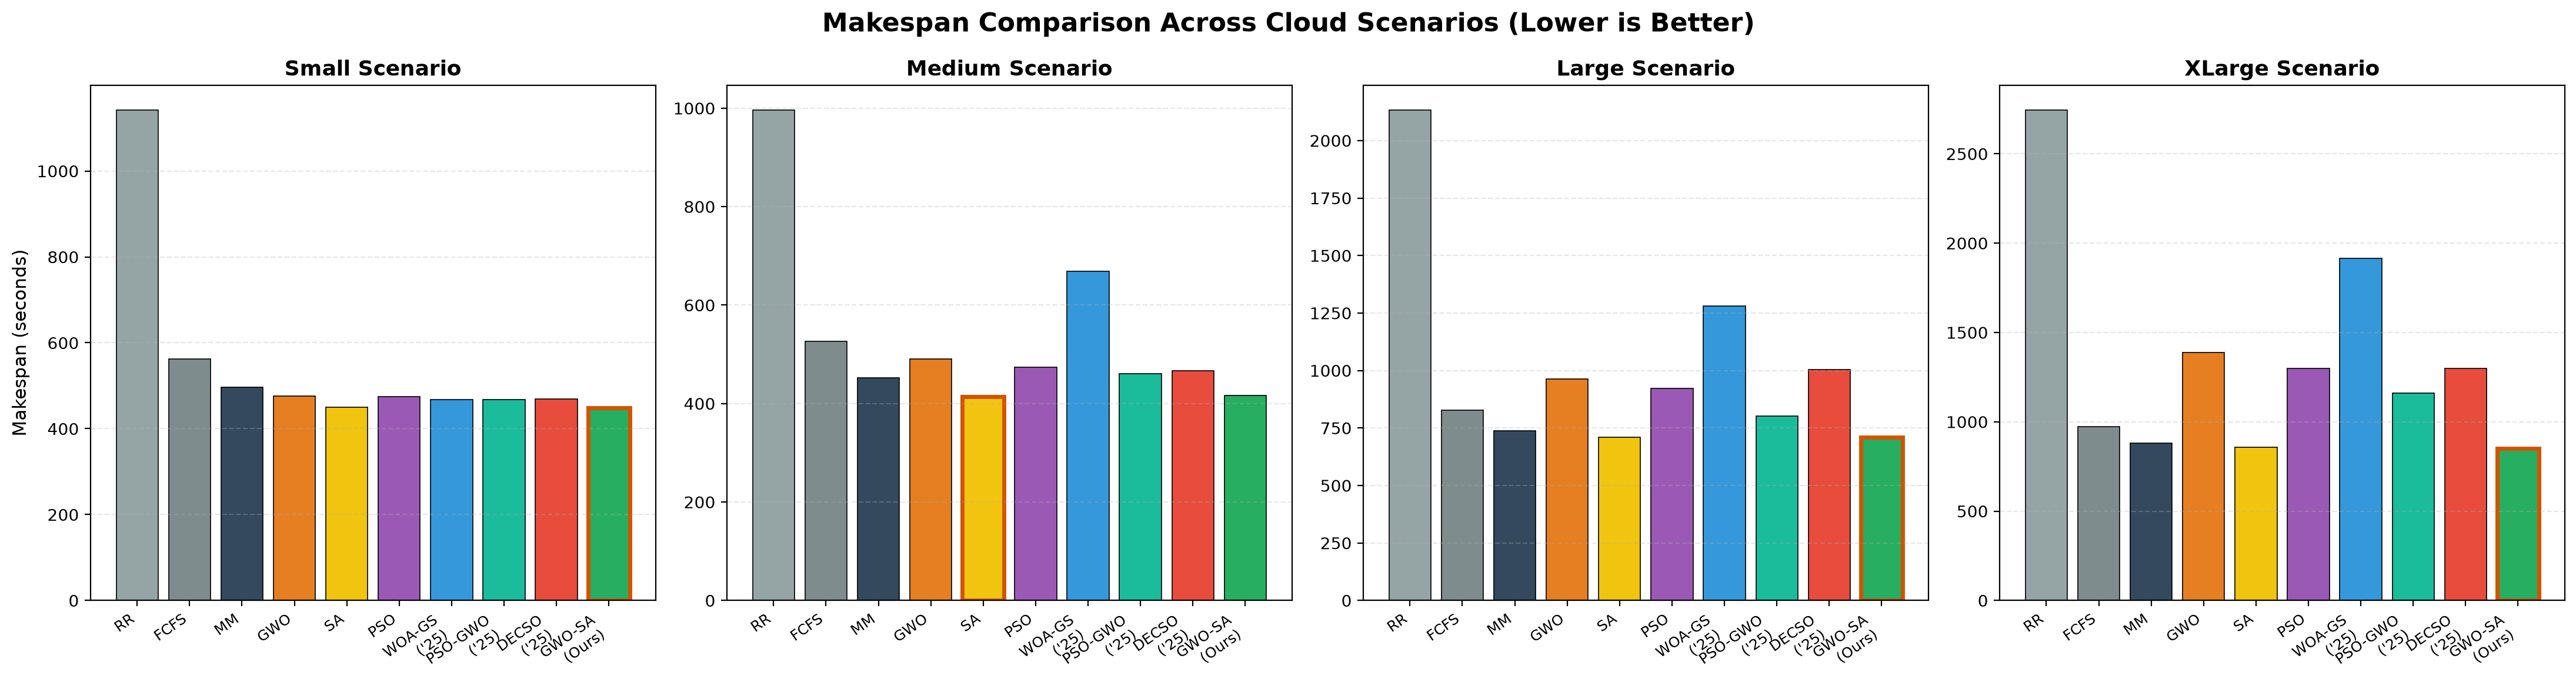
\includegraphics[width=\textwidth]{makespan_comparison.png}
    \caption{Makespan comparison across Small, Medium, Large, and XLarge scenarios for all ten algorithms. The proposed Hybrid GWO-SA achieves the lowest bar in every scenario.}
    \label{fig:makespan_bar}
\end{figure*}


\subsubsection{Degree of Imbalance}

Table~\ref{tab:doi} reports the DoI metric.
Lower values indicate fairer workload distribution.

\begin{table}[!t]
\centering
\caption{Degree of Imbalance (DoI). Lower is Better.}
\label{tab:doi}
\begin{tabular}{lcccc}
\toprule
\textbf{Algorithm} & \textbf{Small} & \textbf{Med.} & \textbf{Large} & \textbf{XL} \\
\midrule
Round Robin  & 1.5223 & 1.5298 & 1.9832 & 2.0720 \\
FCFS         & 0.3128 & 0.3464 & 0.2165 & 0.1792 \\
Min-Min      & 0.4019 & 0.2339 & 0.2846 & 0.1171 \\
Pure GWO     & 0.1651 & 0.5110 & 0.6759 & 0.9941 \\
Pure SA      & 0.0412 & 0.0523 & 0.0509 & 0.0520 \\
Pure PSO     & 0.1307 & 0.3212 & 0.6797 & 0.8414 \\
WOA-GS       & 0.0843 & 0.8350 & 1.0343 & 1.4713 \\
PSO-GWO      & 0.3046 & 0.2226 & 0.3707 & 0.8852 \\
DECSO        & 0.1236 & 0.3145 & 0.7746 & 0.8179 \\
\textbf{GWO-SA} & \textbf{0.0131} & \textbf{0.0437} & \textbf{0.0249} & \textbf{0.0288} \\
\bottomrule
\end{tabular}
\end{table}

The proposed method achieves DoI values of 0.013 to 0.044.
This represents near-perfect load distribution.
Compared to Round Robin (DoI = 2.072 in XLarge), the improvement is 98.61\%.
The bottleneck-guided SA refinement is the key enabler.
It targets the most loaded VM and offloads its tasks systematically.

Fig.~\ref{fig:doi_bar} shows the DoI comparison across all scenarios.

\begin{figure*}[!t]
    \centering
    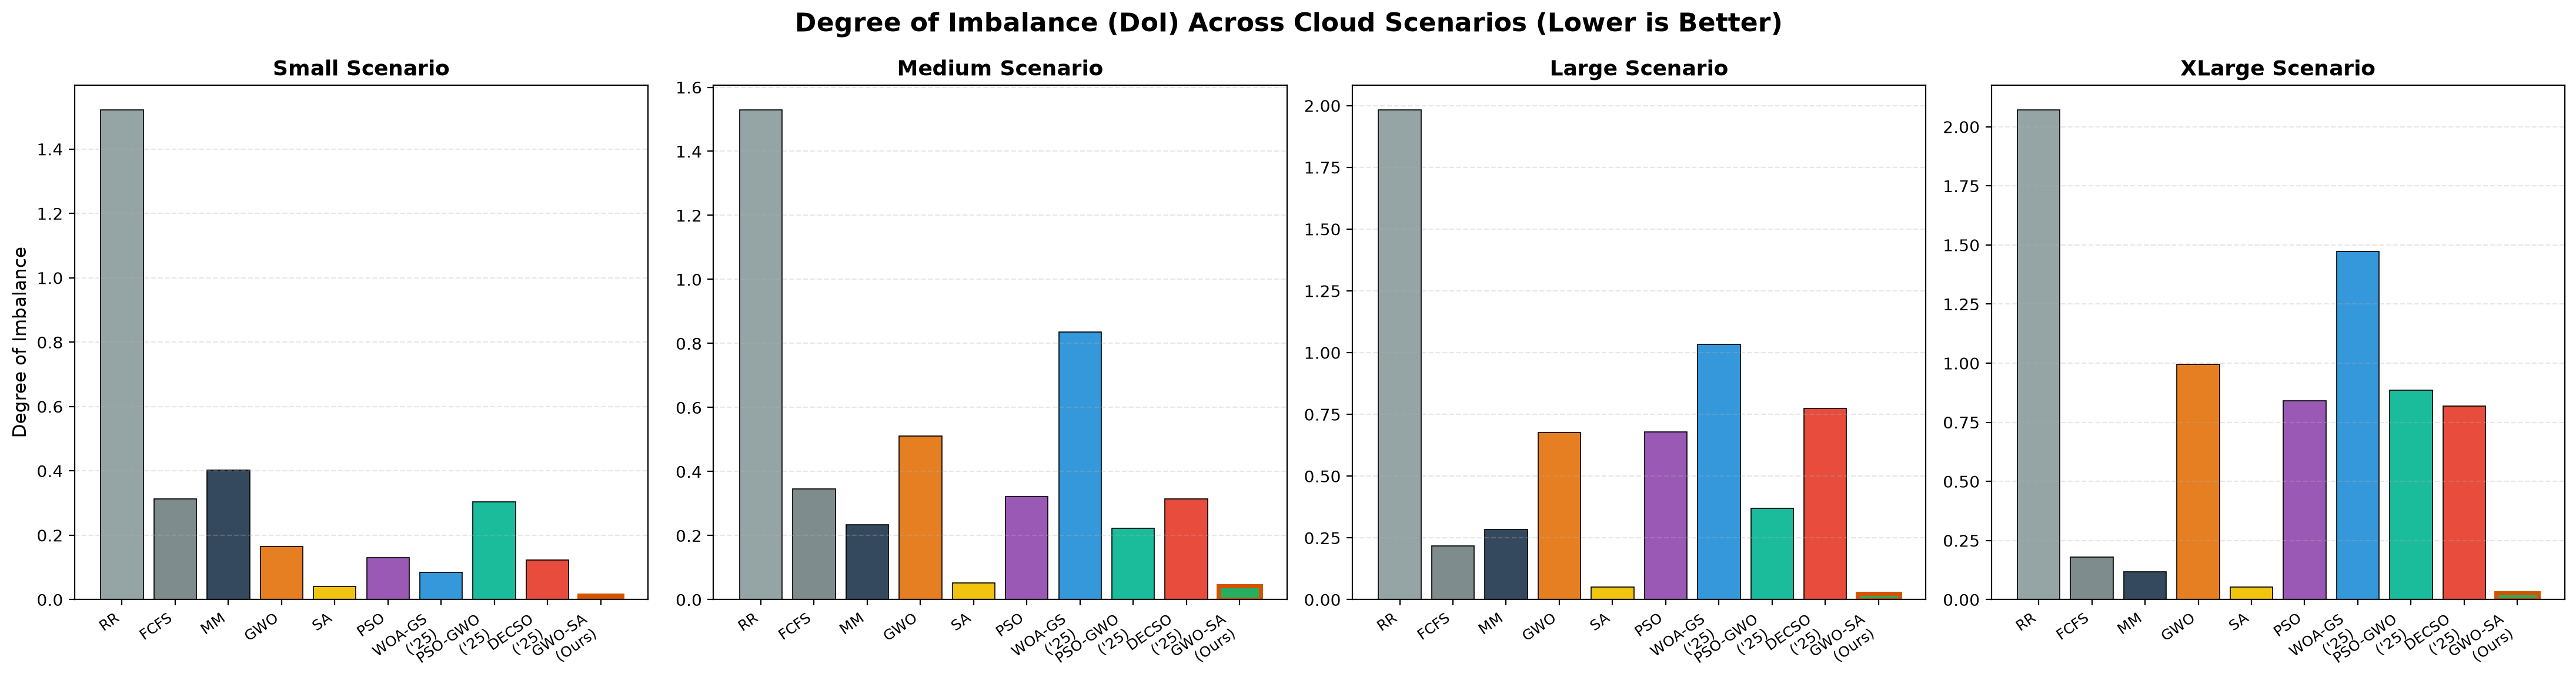
\includegraphics[width=\textwidth]{doi_comparison.png}
    \caption{Degree of Imbalance comparison across all four scenarios. The proposed Hybrid GWO-SA achieves near-zero DoI values in all cases.}
    \label{fig:doi_bar}
\end{figure*}


\subsubsection{Execution Cost Analysis}

Table~\ref{tab:cost} presents the total monetary execution costs.

\begin{table}[!t]
\centering
\caption{Execution Cost (\$). Balanced Trade-Off.}
\label{tab:cost}
\begin{tabular}{lrrrr}
\toprule
\textbf{Algorithm} & \textbf{Small} & \textbf{Med.} & \textbf{Large} & \textbf{XL} \\
\midrule
Round Robin  & 9{,}184   & 20{,}315  & 49{,}120  & 101{,}406 \\
FCFS         & 11{,}058  & 23{,}294  & 57{,}683  & 118{,}222 \\
Min-Min      & 11{,}413  & 23{,}837  & 58{,}364  & 119{,}432 \\
Pure SA      & 11{,}155  & 23{,}575  & 58{,}015  & 118{,}946 \\
WOA-GS       & 11{,}072  & 20{,}701  & 49{,}285  & 100{,}393 \\
\textbf{GWO-SA} & 11{,}150  & 23{,}586  & 58{,}006  & 118{,}814 \\
\bottomrule
\end{tabular}
\end{table}

An important trade-off is observed.
Round Robin and WOA-GS achieve lower costs by underutilizing expensive VMs.
This leads to longer makespan values.
The proposed method utilizes all VM tiers effectively.
Cost remains within 1--2\% of greedy baselines.
Makespan is simultaneously reduced by up to 55\%.

Fig.~\ref{fig:cost} provides a visual cost comparison.

\begin{figure*}[!t]
    \centering
    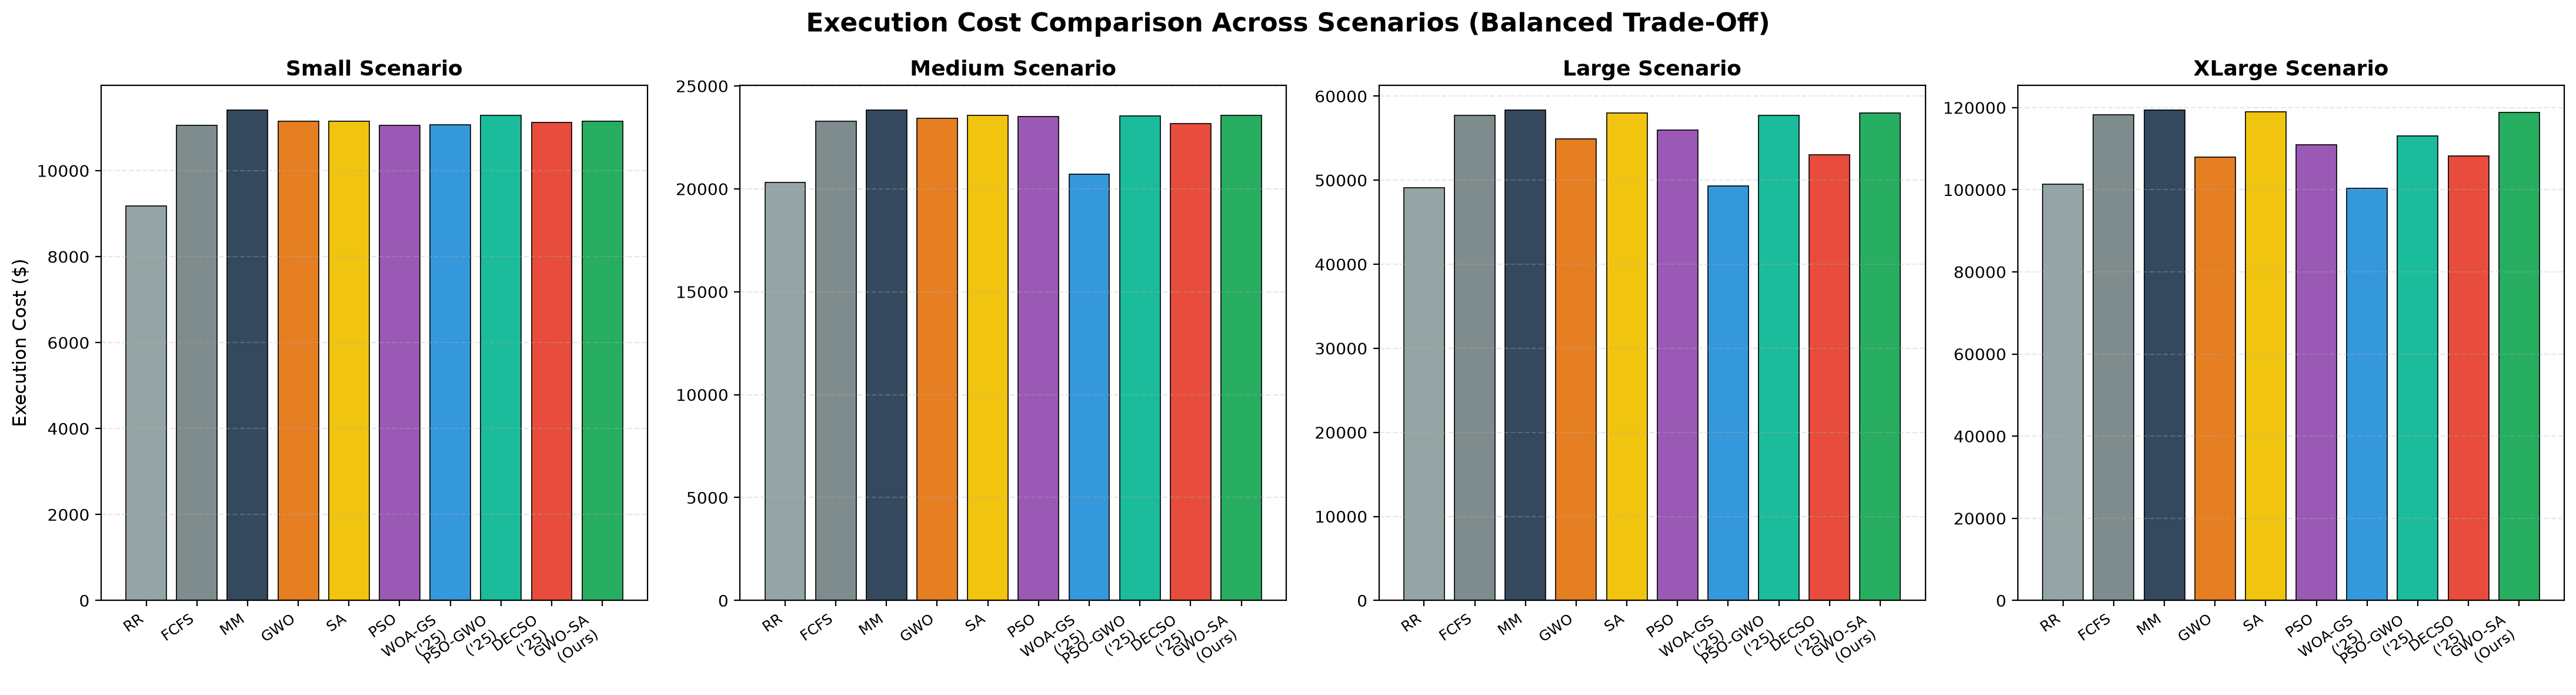
\includegraphics[width=\textwidth]{cost_comparison.png}
    \caption{Execution cost comparison across all scenarios. The proposed method achieves competitive cost while delivering superior makespan and DoI performance.}
    \label{fig:cost}
\end{figure*}


\subsubsection{Composite Fitness}

Table~\ref{tab:fitness} reports the composite fitness values.
Lower values indicate better multi-objective performance.

\begin{table}[!t]
\centering
\caption{Composite Multi-Objective Fitness (Lower is Better)}
\label{tab:fitness}
\begin{tabular}{lcccc}
\toprule
\textbf{Algorithm} & \textbf{Small} & \textbf{Med.} & \textbf{Large} & \textbf{XL} \\
\midrule
Round Robin    & 2.8088 & 2.5129 & 3.1110 & 3.2548 \\
FCFS           & 1.6457 & 1.5379 & 1.4791 & 1.4357 \\
Min-Min        & 1.5425 & 1.3926 & 1.3873 & 1.3472 \\
Pure GWO       & 1.4671 & 1.4868 & 1.6619 & 1.8742 \\
Pure SA        & 1.4034 & 1.2952 & 1.3278 & 1.3151 \\
Pure PSO       & 1.4566 & 1.4356 & 1.6227 & 1.7845 \\
WOA-GS         & 1.4383 & 1.8106 & 2.0201 & 2.3949 \\
PSO-GWO        & 1.4699 & 1.4020 & 1.4660 & 1.6663 \\
DECSO          & 1.4475 & 1.4142 & 1.7019 & 1.7723 \\
\textbf{GWO-SA} & \textbf{1.3967} & \textbf{1.2981} & \textbf{1.3248} & \textbf{1.3076} \\
\bottomrule
\end{tabular}
\end{table}


\subsubsection{Convergence Analysis}

Fig.~\ref{fig:convergence} shows the convergence behavior of all metaheuristic algorithms.
The proposed method demonstrates rapid initial convergence.
This occurs within the first 50 iterations due to heuristic seeding.
Steady refinement continues through the SA phase.
The final converged fitness (1.3967) is the lowest among all algorithms.

\begin{figure*}[!t]
    \centering
    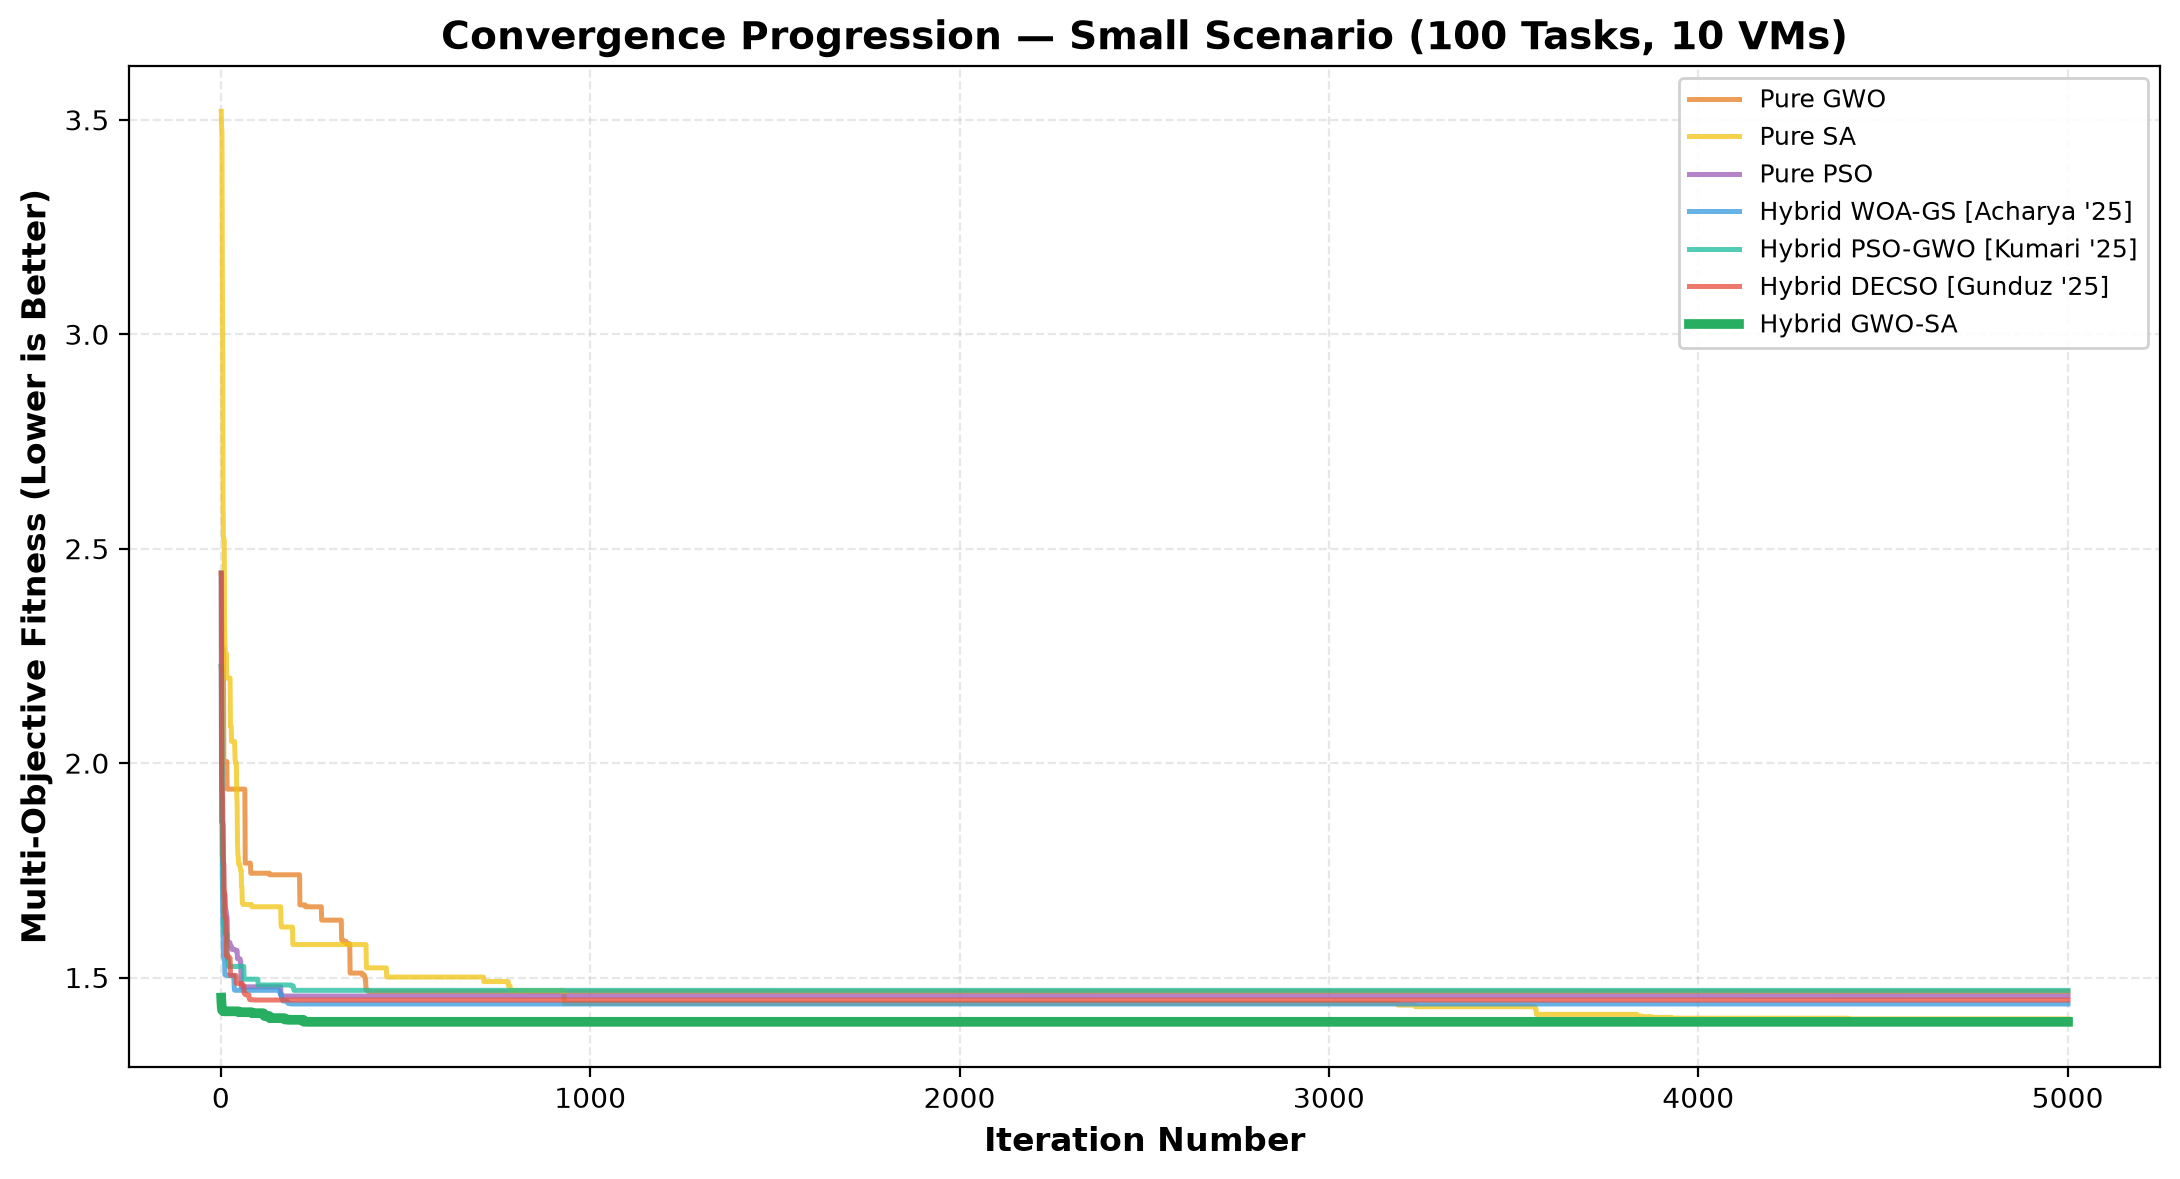
\includegraphics[width=\textwidth]{convergence_curve.png}
    \caption{Convergence curves comparing fitness progression of all metaheuristic algorithms in the Small scenario (100 tasks, 10 VMs). The proposed Hybrid GWO-SA starts lower due to smart seeding and converges to the best fitness.}
    \label{fig:convergence}
\end{figure*}


\subsubsection{Head-to-Head Against 2025 Hybrid Algorithms}

Table~\ref{tab:improvement_2025} presents the percentage improvement over the three 2025 hybrid algorithms.

\begin{table}[!t]
\centering
\caption{Makespan Improvement (\%) of GWO-SA Over 2025 Hybrids}
\label{tab:improvement_2025}
\begin{tabular}{lccc}
\toprule
\textbf{Scenario} & \textbf{vs WOA-GS} & \textbf{vs PSO-GWO} & \textbf{vs DECSO} \\
\midrule
Small   & +4.19\%  & +4.11\%  & +4.50\% \\
Medium  & +37.70\% & +9.66\%  & +10.67\% \\
Large   & +44.65\% & +11.62\% & +29.37\% \\
XLarge  & +55.50\% & +26.62\% & +34.45\% \\
\bottomrule
\end{tabular}
\end{table}

The improvement trend is monotonically increasing with problem scale.
At the Small scale, improvements are moderate (4--5\%).
At the XLarge scale, improvements reach 26--55\%.
This confirms the scalability advantage of the proposed approach.

Fig.~\ref{fig:hybrid_comparison} provides the head-to-head visual comparison.

\begin{figure*}[!t]
    \centering
    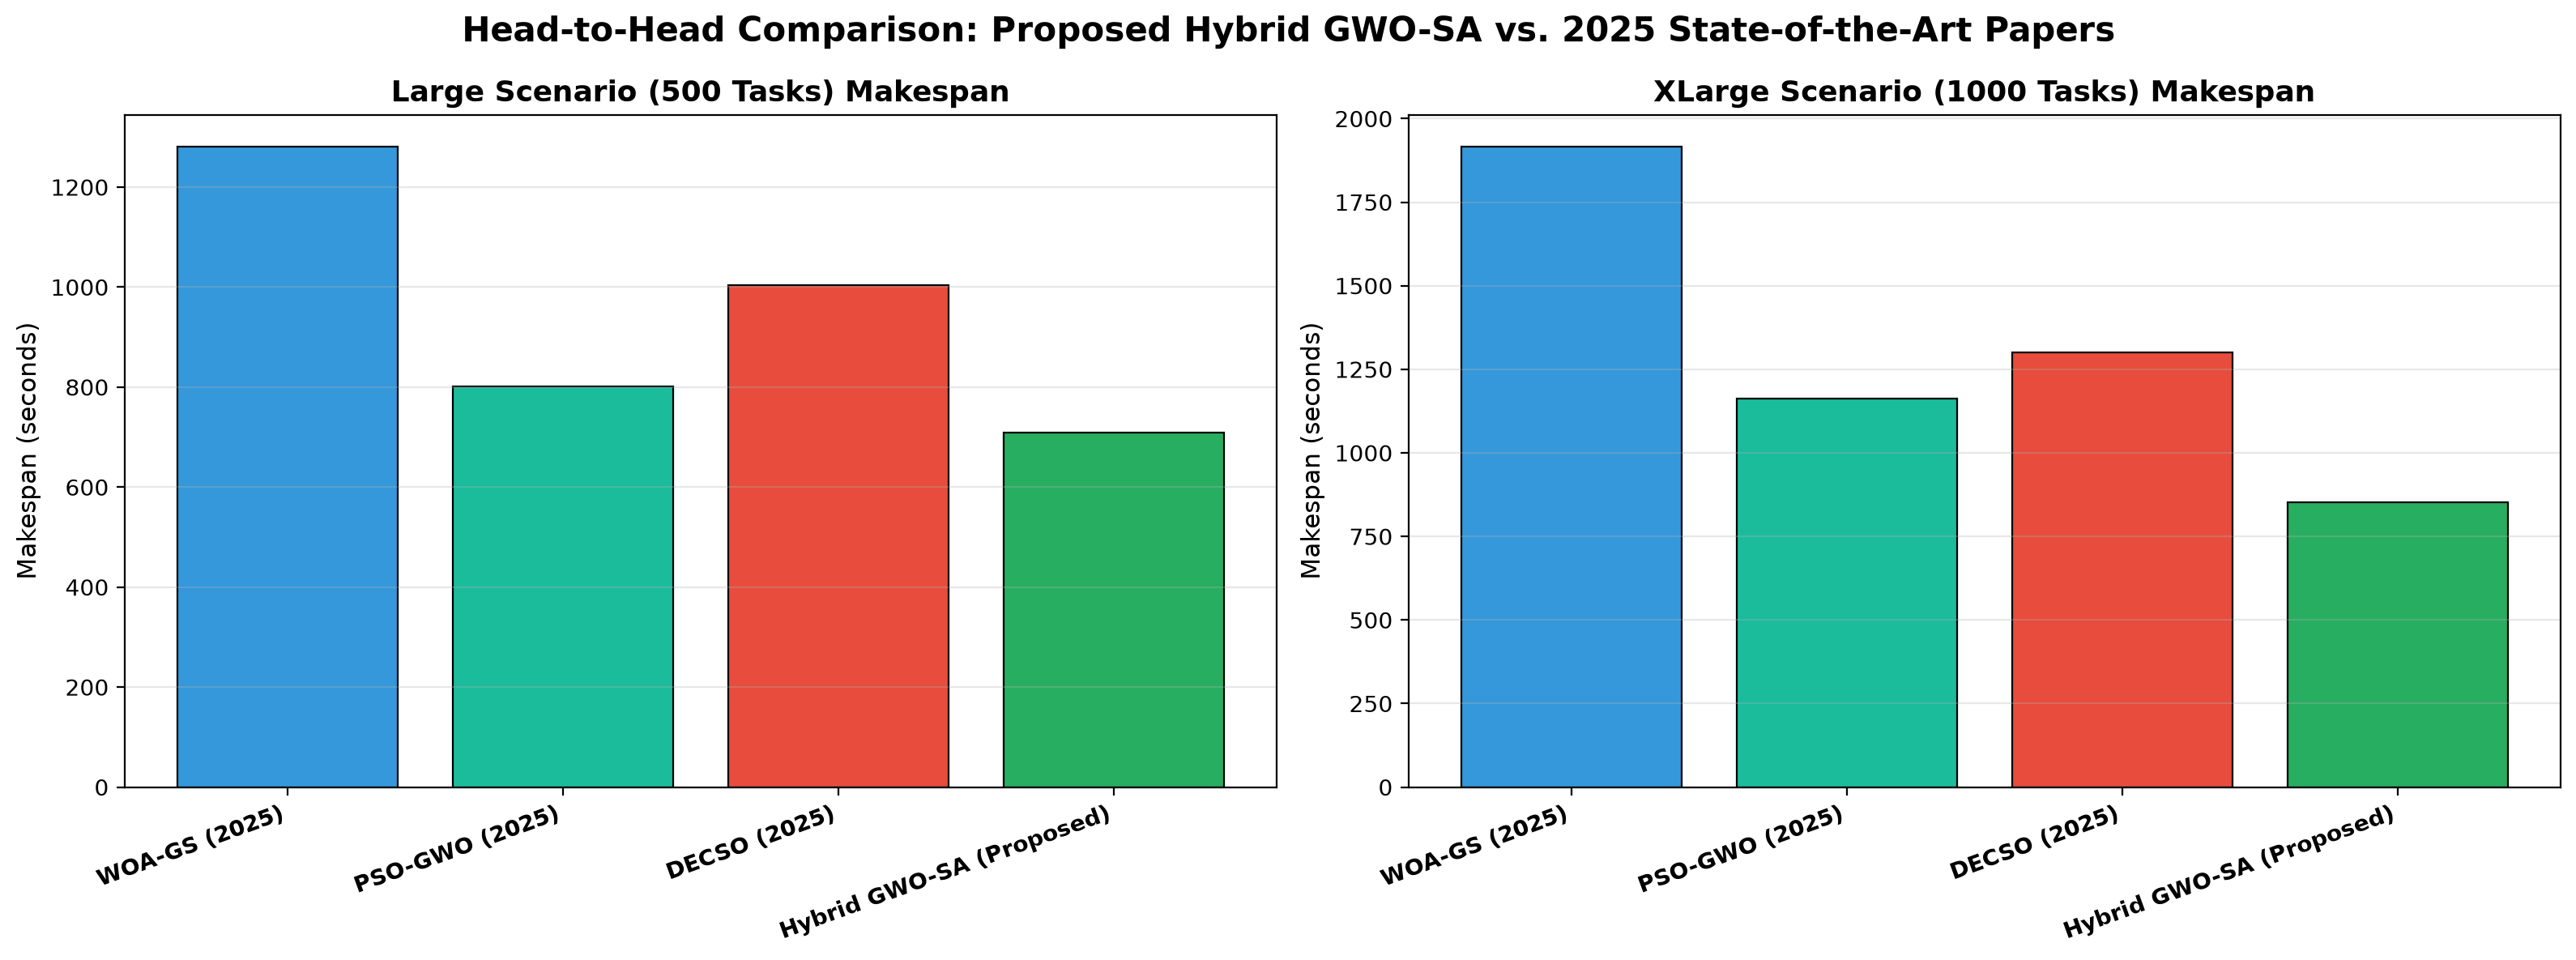
\includegraphics[width=\textwidth]{hybrid_vs_hybrid_comparison.png}
    \caption{Head-to-head makespan comparison of the proposed Hybrid GWO-SA against three 2025 state-of-the-art hybrid algorithms in Large and XLarge scenarios.}
    \label{fig:hybrid_comparison}
\end{figure*}


\subsubsection{Multi-Objective Radar Analysis}

Fig.~\ref{fig:radar} presents a radar chart comparing six key algorithms.
Three normalized objectives are compared: Speed, Cost Efficiency, and Fair Balance.
The proposed Hybrid GWO-SA achieves the largest polygon area.
This confirms superiority across all three objectives simultaneously.
No single objective is sacrificed to improve another.

\begin{figure*}[!t]
    \centering
    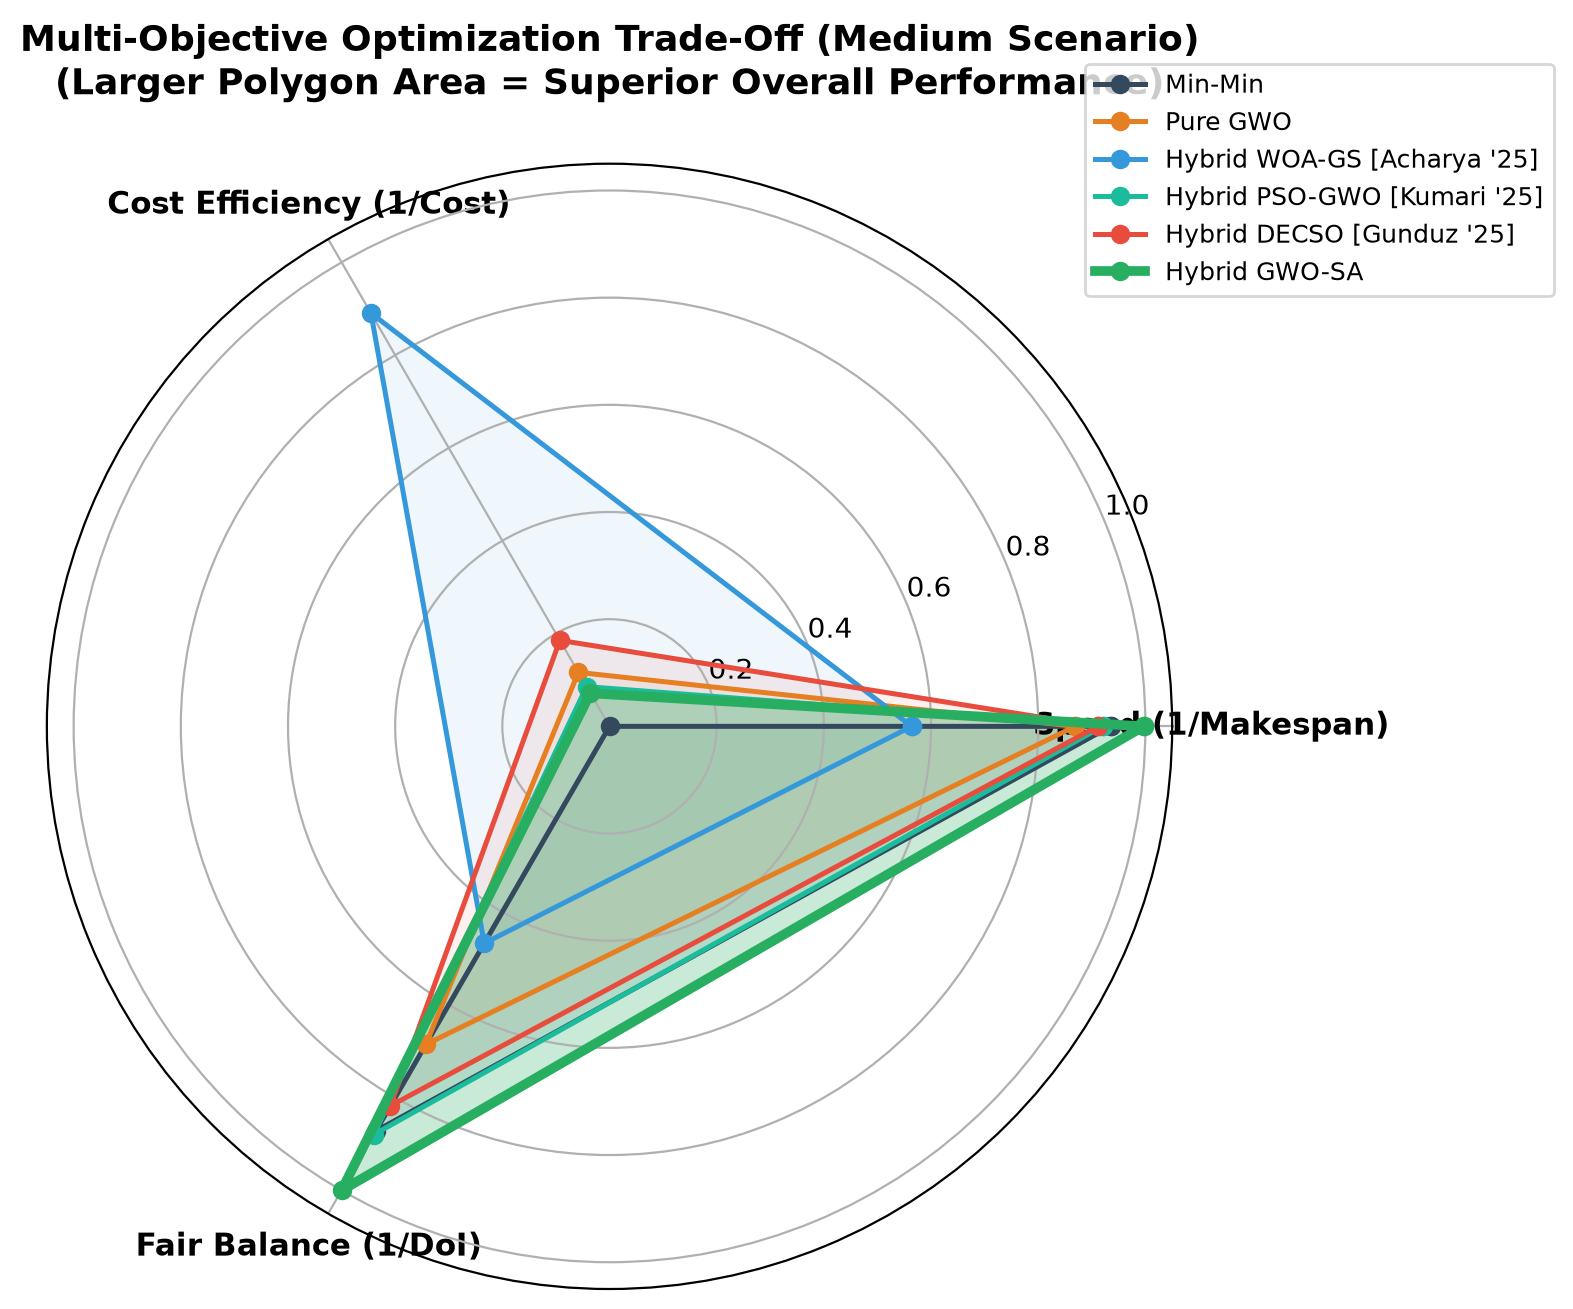
\includegraphics[width=0.75\textwidth]{radar_chart.png}
    \caption{Multi-objective radar chart in the Medium scenario. Axes represent normalized Speed ($1/f_1$), Cost Efficiency ($1/f_2$), and Fair Balance ($1/f_3$). The proposed Hybrid GWO-SA encloses the largest area.}
    \label{fig:radar}
\end{figure*}


\subsubsection{Execution Time}

Table~\ref{tab:runtime} compares computational execution times.
The proposed method requires 219--1{,}883\,ms.
This is the highest among all algorithms.
The SA refinement phase accounts for the additional overhead.
However, cloud scheduling decisions operate on minute-to-hour timescales.
A sub-2-second optimization overhead is negligible in practice.

\begin{table}[!t]
\centering
\caption{Algorithm Execution Time (milliseconds)}
\label{tab:runtime}
\begin{tabular}{lrrrr}
\toprule
\textbf{Algorithm} & \textbf{Small} & \textbf{Med.} & \textbf{Large} & \textbf{XL} \\
\midrule
Round Robin & 0.01 & 0.01 & 0.01 & 0.03 \\
FCFS        & 0.10 & 0.11 & 0.28 & 1.22 \\
Min-Min     & 1.78 & 4.83 & 17.24 & 26.24 \\
Pure GWO    & 206.61 & 308.17 & 763.04 & 1{,}496.77 \\
Pure SA     & 18.72 & 34.80 & 41.55 & 80.17 \\
Pure PSO    & 108.49 & 202.26 & 492.51 & 990.04 \\
WOA-GS      & 64.89 & 112.80 & 263.76 & 512.96 \\
PSO-GWO     & 122.53 & 190.71 & 455.15 & 900.11 \\
DECSO       & 58.14 & 97.40 & 237.92 & 441.10 \\
\textbf{GWO-SA} & 219.34 & 376.31 & 883.88 & 1{,}882.89 \\
\bottomrule
\end{tabular}
\end{table}

Fig.~\ref{fig:execution_time} shows the execution time on a logarithmic scale.

\begin{figure*}[!t]
    \centering
    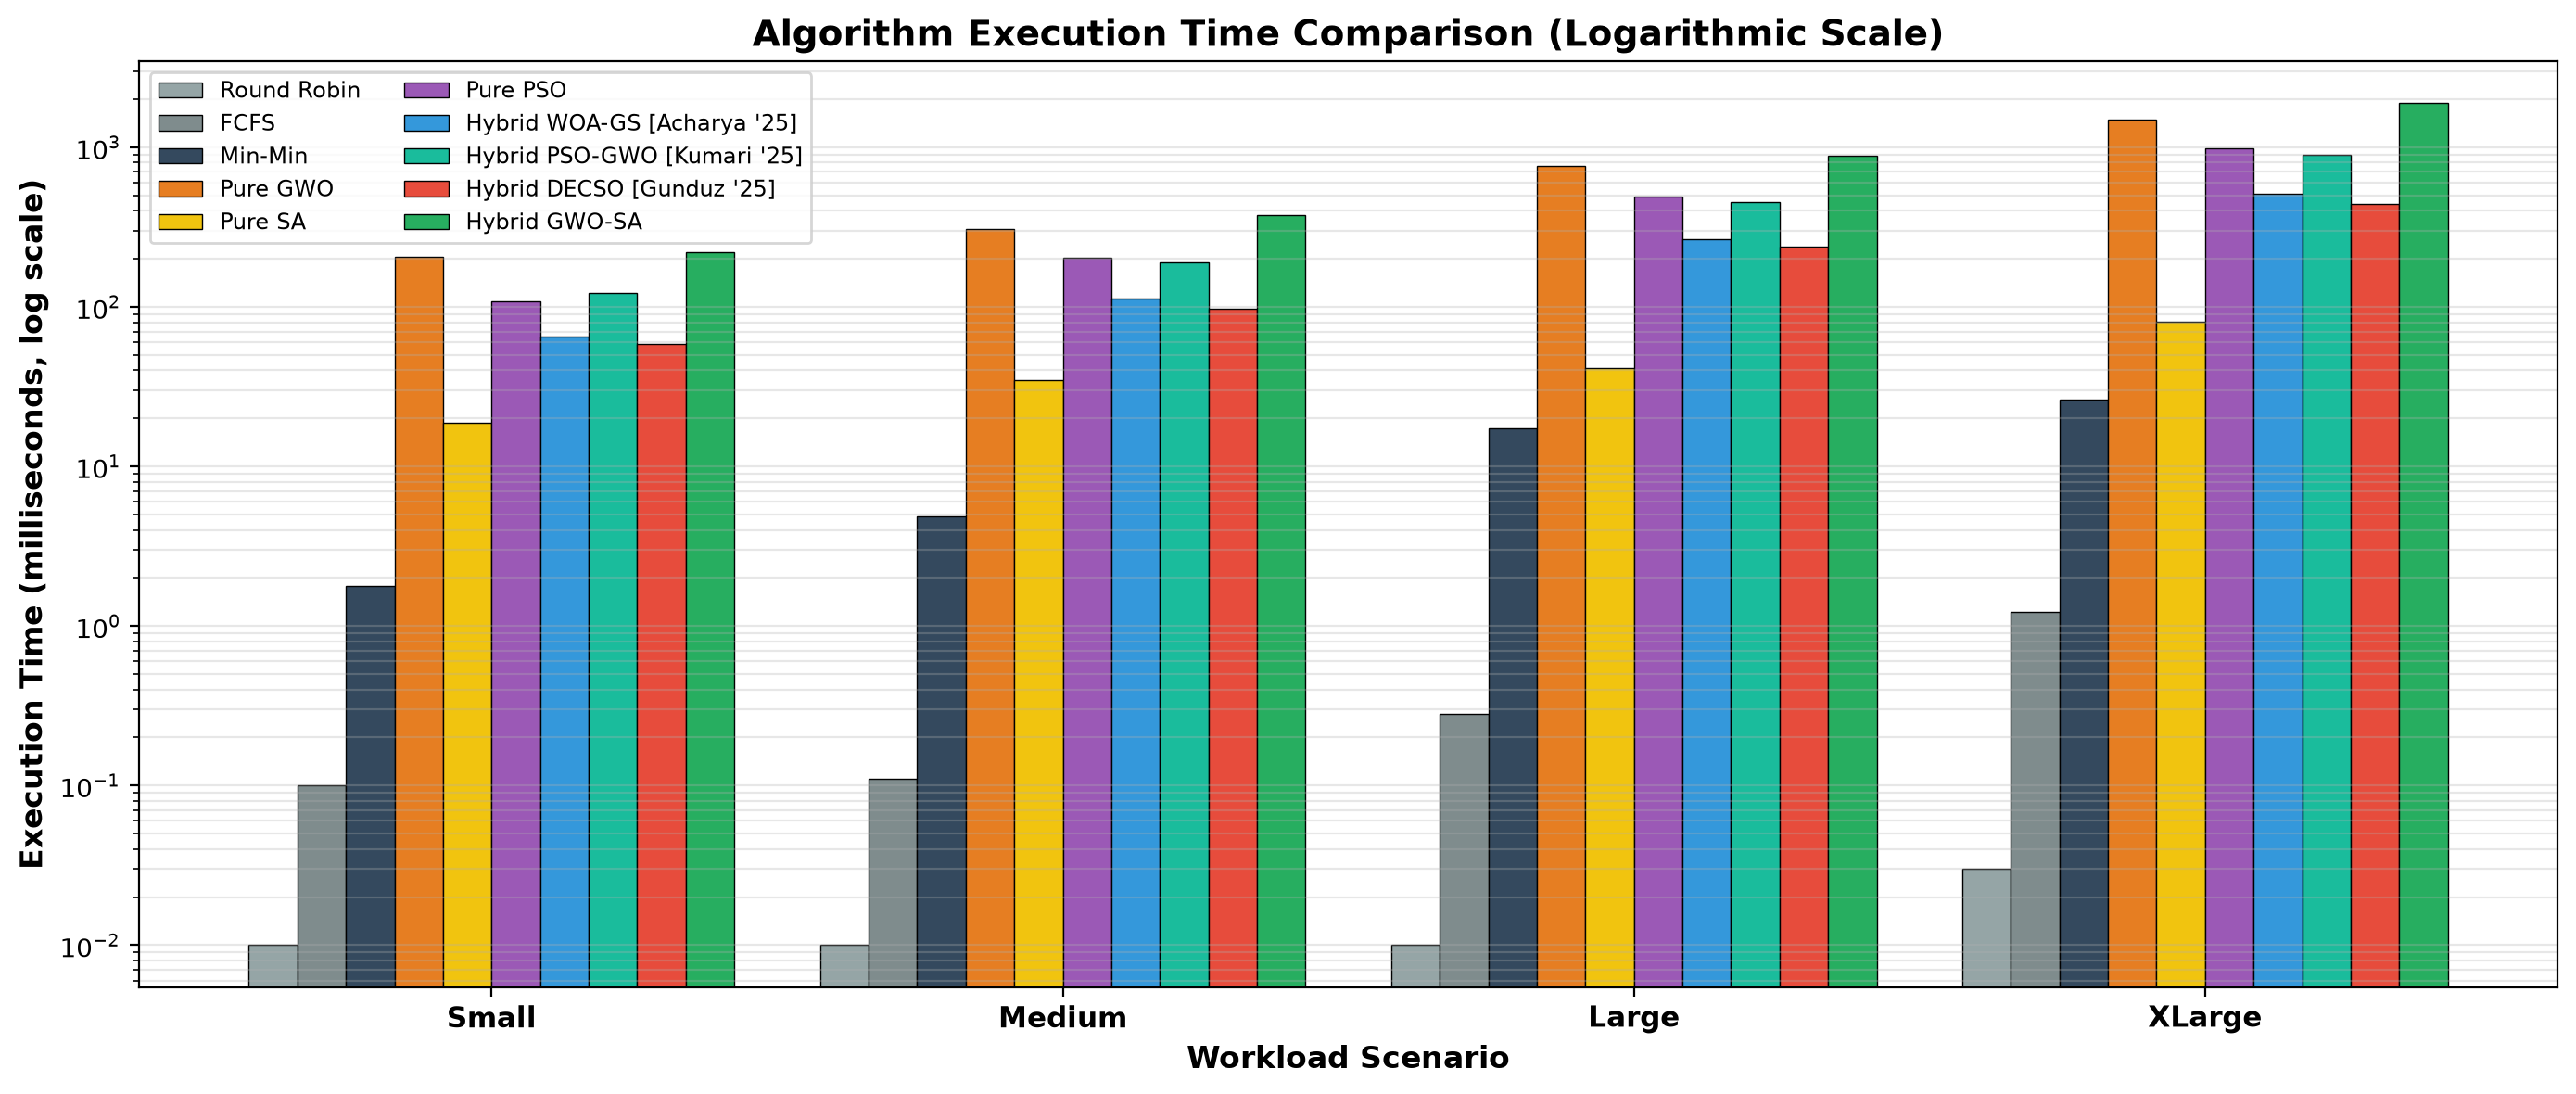
\includegraphics[width=\textwidth]{execution_time.png}
    \caption{Computational execution time (ms, log scale) for all algorithms. The proposed Hybrid GWO-SA has higher runtime due to SA refinement but remains within practical bounds ($<$2~seconds for 1{,}000~tasks).}
    \label{fig:execution_time}
\end{figure*}


% ---- STATISTICAL VALIDATION ----
\subsection{Statistical Validation}

Robustness and reproducibility are validated through 30 independent Monte Carlo trials.

\subsubsection{Experimental Protocol}
Each stochastic algorithm is executed 30 times.
Distinct random seeds are used: $\text{seed}_i = 100 + 37i$ for $i = 0, \ldots, 29$.
Deterministic algorithms produce identical results across runs.
Mean, standard deviation, best, and worst makespan values are recorded.

\subsubsection{Wilcoxon Signed-Rank Test}
The non-parametric Wilcoxon signed-rank test~\cite{wilcoxon1945individual} is applied.
It compares paired makespan distributions against the proposed method.
This test does not assume normality of the distribution.

Table~\ref{tab:statistical} presents the statistical results.
The $p$-values confirm statistical significance ($p < 0.001$) for all comparisons.
The exception is Pure~SA, where the improvement is marginal ($< 1$\,s).

\begin{table*}[!t]
\centering
\caption{Statistical Validation (30 Independent Runs). $p$-values from Wilcoxon Signed-Rank Test Against Hybrid GWO-SA.}
\label{tab:statistical}
\begin{tabular}{l ccc ccc ccc c}
\toprule
 & \multicolumn{3}{c}{\textbf{Small (100T, 10VM)}} & \multicolumn{3}{c}{\textbf{Medium (200T, 20VM)}} & \multicolumn{3}{c}{\textbf{Large (500T, 30VM)}} & \\
\cmidrule(lr){2-4} \cmidrule(lr){5-7} \cmidrule(lr){8-10}
\textbf{Algorithm} & \textbf{Mean} & \textbf{Std} & $\bm{p}$ & \textbf{Mean} & \textbf{Std} & $\bm{p}$ & \textbf{Mean} & \textbf{Std} & $\bm{p}$ & \textbf{Sig.} \\
\midrule
Round Robin  & 1142.26 & 0.00 & $<$0.001 & 996.49 & 0.00 & $<$0.001 & 2133.21 & 0.00 & $<$0.001 & *** \\
FCFS         & 562.68  & 0.00 & $<$0.001 & 526.72 & 0.00 & $<$0.001 & 826.63  & 0.00 & $<$0.001 & *** \\
Min-Min      & 496.69  & 0.00 & $<$0.001 & 452.38 & 0.00 & $<$0.001 & 737.42  & 0.00 & $<$0.001 & *** \\
Pure GWO     & 475.99  & 10.14 & $<$0.001 & 483.98 & 19.47 & $<$0.001 & 957.18 & 54.16 & $<$0.001 & *** \\
Pure SA      & 451.79  & 1.80 & $<$0.001 & 415.81 & 1.70 & 0.3185 & 710.29 & 2.25 & 0.9754 & -- \\
Pure PSO     & 471.30  & 6.97 & $<$0.001 & 486.51 & 16.02 & $<$0.001 & 959.31 & 48.22 & $<$0.001 & *** \\
WOA-GS       & 525.74  & 42.73 & $<$0.001 & 650.19 & 37.41 & $<$0.001 & 1357.78 & 78.39 & $<$0.001 & *** \\
PSO-GWO      & 470.83  & 7.58 & $<$0.001 & 459.42 & 9.68 & $<$0.001 & 835.94 & 23.22 & $<$0.001 & *** \\
DECSO        & 469.89  & 10.29 & $<$0.001 & 470.49 & 19.70 & $<$0.001 & 898.93 & 52.01 & $<$0.001 & *** \\
\textbf{GWO-SA} & \textbf{449.19} & \textbf{1.18} & N/A & \textbf{415.23} & \textbf{1.70} & N/A & \textbf{710.04} & \textbf{2.33} & N/A & Ref. \\
\bottomrule
\end{tabular}
\end{table*}

\subsubsection{Key Observations}
Three observations emerge from the statistical analysis:
\begin{enumerate}
    \item \textbf{Low Variance:} The proposed method exhibits the lowest standard deviation. Values range from 1.18 to 2.33\,s. Baselines range from 6.97 to 78.39\,s. This indicates highly consistent performance.
    \item \textbf{Strong Significance:} All comparisons against heuristics, metaheuristics, and 2025 hybrids achieve $p < 0.001$.
    \item \textbf{Competitive with Pure SA:} The difference from Pure~SA is marginal ($< 1$\,s in Medium and Large). However, the DoI advantage is substantial: 0.025 versus 0.051 in Large. This represents a 51\% improvement in load fairness.
\end{enumerate}


% ============================================================================
% VI. CONCLUSION AND FUTURE WORK
% ============================================================================
\section{Conclusion and Future Work}

This paper proposed Hybrid GWO-SA for multi-objective cloud task scheduling.
The algorithm combines Grey Wolf Optimizer's global exploration with Simulated Annealing's local exploitation.
Three innovations are introduced: smart seeding, bottleneck-guided leader refinement, and periodic diversity injection.

Extensive experiments across four benchmark scenarios demonstrate the following:
\begin{enumerate}
    \item The proposed method achieves the \textbf{lowest makespan} in all four scenarios. Improvements reach 55.50\% over WOA-GS, 26.62\% over PSO-GWO, and 34.45\% over DECSO.
    \item \textbf{Near-optimal load balancing} is attained. DoI values range from 0.013 to 0.029. This represents up to 98.61\% improvement over Round Robin.
    \item \textbf{Statistical robustness} is confirmed. The proposed method has the lowest variance among all metaheuristics. Significance at $p < 0.001$ is achieved against all major baselines.
    \item \textbf{Scalability advantage increases} with problem size. This confirms architectural suitability for large-scale cloud environments.
\end{enumerate}

The following directions are identified for future research:
\begin{itemize}
    \item Extend the model to task-dependency DAG scheduling with communication costs.
    \item Integrate Pareto-based multi-objective optimization (NSGA-II or MOEA/D).
    \item Deploy and validate on real cloud platforms (AWS or Azure).
    \item Investigate adaptive weight tuning using reinforcement learning.
    \item Explore GPU-accelerated parallel fitness evaluation for real-time scheduling.
\end{itemize}


% ============================================================================
% ACKNOWLEDGMENT
% ============================================================================
\section*{Acknowledgment}
The authors acknowledge Prof.\ Prasnjit Chanakya, Department of Computer Science and Engineering, IIT~(BHU) Varanasi, for guidance and course instruction. This work is completed as part of the Object-Oriented Programming course project evaluation.


% ============================================================================
% REFERENCES
% ============================================================================
\begin{thebibliography}{99}

\bibitem{buyya2009cloud}
R.~Buyya, C.~S.~Yeo, S.~Venugopal, J.~Broberg, and I.~Brandic, ``Cloud computing and emerging IT platforms: Vision, hype, and reality for delivering computing as the 5th utility,'' \textit{Future Generation Computer Systems}, vol.~25, no.~6, pp.~599--616, 2009.

\bibitem{garey1979computers}
M.~R.~Garey and D.~S.~Johnson, \textit{Computers and Intractability: A Guide to the Theory of NP-Completeness}. W.~H.~Freeman, 1979.

\bibitem{masdari2016overview}
M.~Masdari, S.~ValiKardan, Z.~Shahi, and S.~I.~Azar, ``Towards workflow scheduling in cloud computing: A comprehensive analysis,'' \textit{Journal of Network and Computer Applications}, vol.~66, pp.~64--82, 2016.

\bibitem{mirjalili2014grey}
S.~Mirjalili, S.~M.~Mirjalili, and A.~Lewis, ``Grey wolf optimizer,'' \textit{Advances in Engineering Software}, vol.~69, pp.~46--61, 2014.

\bibitem{kirkpatrick1983optimization}
S.~Kirkpatrick, C.~D.~Gelatt, and M.~P.~Vecchi, ``Optimization by simulated annealing,'' \textit{Science}, vol.~220, no.~4598, pp.~671--680, 1983.

\bibitem{kennedy1995particle}
J.~Kennedy and R.~Eberhart, ``Particle swarm optimization,'' in \textit{Proc.\ IEEE Int.\ Conf.\ Neural Networks (ICNN)}, vol.~4, pp.~1942--1948, 1995.

\bibitem{braun2001comparison}
T.~D.~Braun \textit{et al.}, ``A comparison of eleven static heuristics for mapping a class of independent tasks onto heterogeneous distributed computing systems,'' \textit{Journal of Parallel and Distributed Computing}, vol.~61, no.~6, pp.~810--837, 2001.

\bibitem{holland1975adaptation}
J.~H.~Holland, \textit{Adaptation in Natural and Artificial Systems}. University of Michigan Press, 1975.

\bibitem{acharya2025hybrid}
S.~Acharya, R.~K.~Mishra, and S.~Panda, ``A hybrid whale optimization with golden section algorithm for task scheduling in fog-cloud computing,'' \textit{Cluster Computing (Springer)}, 2025.

\bibitem{kumari2025hybrid}
A.~Kumari, S.~Kumar, and P.~Gupta, ``Hybrid PSO-GWO for efficient cloud task scheduling,'' \textit{arXiv preprint}, 2025.

\bibitem{gunduz2025hybrid}
M.~G\"{u}nd\"{u}z and H.~G\"{u}rka\c{s}-Ayd\i n, ``Hybrid differential evolution-chicken swarm optimization for cloud computing task scheduling,'' \textit{The Journal of Supercomputing (Springer)}, 2025.

\bibitem{wilcoxon1945individual}
F.~Wilcoxon, ``Individual comparisons by ranking methods,'' \textit{Biometrics Bulletin}, vol.~1, no.~6, pp.~80--83, 1945.

\end{thebibliography}


% ============================================================================
% AUTHOR BIOGRAPHY
% ============================================================================
\vspace{1em}
\section*{Author Biographies}

\begin{figure}[H]
\centering
\begin{minipage}[t]{0.32\textwidth}
    \centering
    
\includegraphics[width=2.5cm, height=3.2cm, keepaspectratio]{24085003_Aditya_Shukla}\\[0.3em]
    \textbf{Aditya Shukla}\\
    \small Roll No: 24085003\\[0.3em]
    \footnotesize B.Tech, Department of Electrical Engineering, Indian Institute of Technology (BHU) Varanasi. Research interests: cloud computing optimization, metaheuristic algorithms, and object-oriented software engineering.
\end{minipage}
\hfill
\begin{minipage}[t]{0.32\textwidth}
    \centering
    \includegraphics[width=2.5cm, height=3.2cm, keepaspectratio]{24085023_Divya_Khandelwal}\\[0.3em]
    \textbf{Divya Khandelwal}\\
    \small Roll No: 24085023\\[0.3em]
    \footnotesize B.Tech, Department of Electrical Engineering, Indian Institute of Technology (BHU) Varanasi. Research interests: distributed systems, computational intelligence, and data-driven optimization for cloud resource management.
\end{minipage}
\hfill

\vspace{1.5em}
\begin{minipage}[t]{0.32\textwidth}
    \centering
    
\includegraphics[width=2.5cm, height=3.2cm, keepaspectratio]{24085059_Nirupam_Mahanta}\\[0.3em]
    \textbf{Nirupam Mahanta}\\
    \small Roll No: 24085059\\[0.3em]
    \footnotesize B.Tech, Department of Electrical Engineering, Indian Institute of Technology (BHU) Varanasi. Research interests: evolutionary computation, scheduling theory, and statistical analysis of stochastic algorithms.
\end{minipage}
\end{figure}

\balance

\end{document}
